\documentclass[1p]{elsarticle_modified}
%\bibliographystyle{elsarticle-num}

%\usepackage[colorlinks]{hyperref}
%\usepackage{abbrmath_seonhwa} %\Abb, \Ascr, \Acal ,\Abf, \Afrak
\usepackage{amsfonts}
\usepackage{amssymb}
\usepackage{amsmath}
\usepackage{amsthm}
\usepackage{scalefnt}
\usepackage{amsbsy}
\usepackage{kotex}
\usepackage{caption}
\usepackage{subfig}
\usepackage{color}
\usepackage{graphicx}
\usepackage{xcolor} %% white, black, red, green, blue, cyan, magenta, yellow
\usepackage{float}
\usepackage{setspace}
\usepackage{hyperref}

\usepackage{tikz}
\usetikzlibrary{arrows}

\usepackage{multirow}
\usepackage{array} % fixed length table
\usepackage{hhline}

%%%%%%%%%%%%%%%%%%%%%
\makeatletter
\renewcommand*\env@matrix[1][\arraystretch]{%
	\edef\arraystretch{#1}%
	\hskip -\arraycolsep
	\let\@ifnextchar\new@ifnextchar
	\array{*\c@MaxMatrixCols c}}
\makeatother %https://tex.stackexchange.com/questions/14071/how-can-i-increase-the-line-spacing-in-a-matrix
%%%%%%%%%%%%%%%

\usepackage[normalem]{ulem}

\newcommand{\msout}[1]{\ifmmode\text{\sout{\ensuremath{#1}}}\else\sout{#1}\fi}
%SOURCE: \msout is \stkout macro in https://tex.stackexchange.com/questions/20609/strikeout-in-math-mode

\newcommand{\cancel}[1]{
	\ifmmode
	{\color{red}\msout{#1}}
	\else
	{\color{red}\sout{#1}}
	\fi
}

\newcommand{\add}[1]{
	{\color{blue}\uwave{#1}}
}

\newcommand{\replace}[2]{
	\ifmmode
	{\color{red}\msout{#1}}{\color{blue}\uwave{#2}}
	\else
	{\color{red}\sout{#1}}{\color{blue}\uwave{#2}}
	\fi
}

\newcommand{\Sol}{\mathcal{S}} %segment
\newcommand{\D}{D} %diagram
\newcommand{\A}{\mathcal{A}} %arc


%%%%%%%%%%%%%%%%%%%%%%%%%%%%%5 test

\def\sl{\operatorname{\textup{SL}}(2,\Cbb)}
\def\psl{\operatorname{\textup{PSL}}(2,\Cbb)}
\def\quan{\mkern 1mu \triangleright \mkern 1mu}

\theoremstyle{definition}
\newtheorem{thm}{Theorem}[section]
\newtheorem{prop}[thm]{Proposition}
\newtheorem{lem}[thm]{Lemma}
\newtheorem{ques}[thm]{Question}
\newtheorem{cor}[thm]{Corollary}
\newtheorem{defn}[thm]{Definition}
\newtheorem{exam}[thm]{Example}
\newtheorem{rmk}[thm]{Remark}
\newtheorem{alg}[thm]{Algorithm}

\newcommand{\I}{\sqrt{-1}}
\begin{document}

%\begin{frontmatter}
%
%\title{Boundary parabolic representations of knots up to 8 crossings}
%
%%% Group authors per affiliation:
%\author{Yunhi Cho} 
%\address{Department of Mathematics, University of Seoul, Seoul, Korea}
%\ead{yhcho@uos.ac.kr}
%
%
%\author{Seonhwa Kim} %\fnref{s_kim}}
%\address{Center for Geometry and Physics, Institute for Basic Science, Pohang, 37673, Korea}
%\ead{ryeona17@ibs.re.kr}
%
%\author{Hyuk Kim}
%\address{Department of Mathematical Sciences, Seoul National University, Seoul 08826, Korea}
%\ead{hyukkim@snu.ac.kr}
%
%\author{Seokbeom Yoon}
%\address{Department of Mathematical Sciences, Seoul National University, Seoul, 08826,  Korea}
%\ead{sbyoon15@snu.ac.kr}
%
%\begin{abstract}
%We find all boundary parabolic representation of knots up to 8 crossings.
%
%\end{abstract}
%\begin{keyword}
%    \MSC[2010] 57M25 
%\end{keyword}
%
%\end{frontmatter}

%\linenumbers
%\tableofcontents
%
\newcommand\colored[1]{\textcolor{white}{\rule[-0.35ex]{0.8em}{1.4ex}}\kern-0.8em\color{red} #1}%
%\newcommand\colored[1]{\textcolor{white}{ #1}\kern-2.17ex	\textcolor{white}{ #1}\kern-1.81ex	\textcolor{white}{ #1}\kern-2.15ex\color{red}#1	}

{\Large $\underline{12a_{0987}~(K12a_{0987})}$}

\setlength{\tabcolsep}{10pt}
\renewcommand{\arraystretch}{1.6}
\vspace{1cm}\begin{tabular}{m{100pt}>{\centering\arraybackslash}m{274pt}}
\multirow{5}{120pt}{
	\centering
	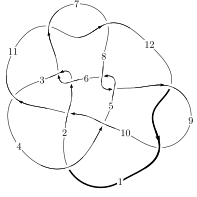
\includegraphics[width=112pt]{../../../GIT/diagram.site/Diagrams/png/1788_12a_0987.png}\\
\ \ \ A knot diagram\footnotemark}&
\allowdisplaybreaks
\textbf{Linearized knot diagam} \\
\cline{2-2}
 &
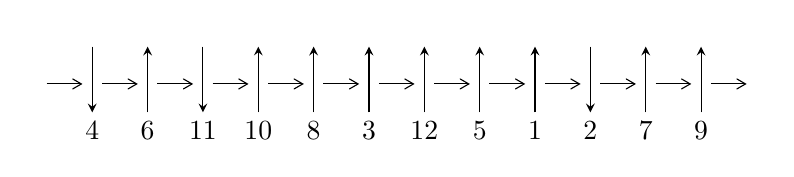
\begin{tikzpicture}[x=20pt, y=17pt]
	% nodes
	\node (C0) at (0, 0) {};
	\node (C1) at (1, 0) {};
	\node (C1U) at (1, +1) {};
	\node (C1D) at (1, -1) {4};

	\node (C2) at (2, 0) {};
	\node (C2U) at (2, +1) {};
	\node (C2D) at (2, -1) {6};

	\node (C3) at (3, 0) {};
	\node (C3U) at (3, +1) {};
	\node (C3D) at (3, -1) {11};

	\node (C4) at (4, 0) {};
	\node (C4U) at (4, +1) {};
	\node (C4D) at (4, -1) {10};

	\node (C5) at (5, 0) {};
	\node (C5U) at (5, +1) {};
	\node (C5D) at (5, -1) {8};

	\node (C6) at (6, 0) {};
	\node (C6U) at (6, +1) {};
	\node (C6D) at (6, -1) {3};

	\node (C7) at (7, 0) {};
	\node (C7U) at (7, +1) {};
	\node (C7D) at (7, -1) {12};

	\node (C8) at (8, 0) {};
	\node (C8U) at (8, +1) {};
	\node (C8D) at (8, -1) {5};

	\node (C9) at (9, 0) {};
	\node (C9U) at (9, +1) {};
	\node (C9D) at (9, -1) {1};

	\node (C10) at (10, 0) {};
	\node (C10U) at (10, +1) {};
	\node (C10D) at (10, -1) {2};

	\node (C11) at (11, 0) {};
	\node (C11U) at (11, +1) {};
	\node (C11D) at (11, -1) {7};

	\node (C12) at (12, 0) {};
	\node (C12U) at (12, +1) {};
	\node (C12D) at (12, -1) {9};
	\node (C13) at (13, 0) {};

	% arrows
	\draw[->,>={angle 60}]
	(C0) edge (C1) (C1) edge (C2) (C2) edge (C3) (C3) edge (C4) (C4) edge (C5) (C5) edge (C6) (C6) edge (C7) (C7) edge (C8) (C8) edge (C9) (C9) edge (C10) (C10) edge (C11) (C11) edge (C12) (C12) edge (C13) ;	\draw[->,>=stealth]
	(C1U) edge (C1D) (C2D) edge (C2U) (C3U) edge (C3D) (C4D) edge (C4U) (C5D) edge (C5U) (C6D) edge (C6U) (C7D) edge (C7U) (C8D) edge (C8U) (C9D) edge (C9U) (C10U) edge (C10D) (C11D) edge (C11U) (C12D) edge (C12U) ;
	\end{tikzpicture} \\
\hhline{~~} \\& 
\textbf{Solving Sequence} \\ \cline{2-2} 
 &
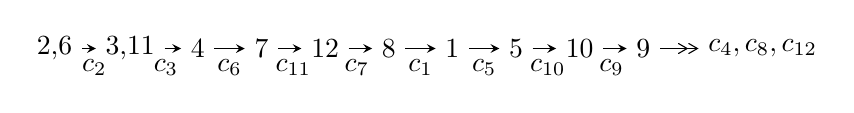
\begin{tikzpicture}[x=23pt, y=7pt]
	% node
	\node (A0) at (-1/8, 0) {2,6};
	\node (A1) at (17/16, 0) {3,11};
	\node (A2) at (17/8, 0) {4};
	\node (A3) at (25/8, 0) {7};
	\node (A4) at (33/8, 0) {12};
	\node (A5) at (41/8, 0) {8};
	\node (A6) at (49/8, 0) {1};
	\node (A7) at (57/8, 0) {5};
	\node (A8) at (65/8, 0) {10};
	\node (A9) at (73/8, 0) {9};
	\node (C1) at (1/2, -1) {$c_{2}$};
	\node (C2) at (13/8, -1) {$c_{3}$};
	\node (C3) at (21/8, -1) {$c_{6}$};
	\node (C4) at (29/8, -1) {$c_{11}$};
	\node (C5) at (37/8, -1) {$c_{7}$};
	\node (C6) at (45/8, -1) {$c_{1}$};
	\node (C7) at (53/8, -1) {$c_{5}$};
	\node (C8) at (61/8, -1) {$c_{10}$};
	\node (C9) at (69/8, -1) {$c_{9}$};
	\node (A10) at (11, 0) {$c_{4},c_{8},c_{12}$};

	% edge
	\draw[->,>=stealth]	
	(A0) edge (A1) (A1) edge (A2) (A2) edge (A3) (A3) edge (A4) (A4) edge (A5) (A5) edge (A6) (A6) edge (A7) (A7) edge (A8) (A8) edge (A9) ;
	\draw[->>,>={angle 60}]	
	(A9) edge (A10);
\end{tikzpicture} \\ 

\end{tabular} \\

\footnotetext{
The image of knot diagram is generated by the software ``\textbf{Draw programme}" developed by Andrew Bartholomew(\url{http://www.layer8.co.uk/maths/draw/index.htm\#Running-draw}), where we modified some parts for our purpose(\url{https://github.com/CATsTAILs/LinksPainter}).
}\phantom \\ \newline 
\centering \textbf{Ideals for irreducible components\footnotemark of $X_{\text{par}}$} 
 
\begin{align*}
I^u_{1}&=\langle 
1.86463\times10^{467} u^{122}-1.08545\times10^{468} u^{121}+\cdots+8.79558\times10^{470} b+5.71526\times10^{472},\\
\phantom{I^u_{1}}&\phantom{= \langle  }7.73571\times10^{471} u^{122}-5.76169\times10^{472} u^{121}+\cdots+7.85533\times10^{474} a-1.00953\times10^{477},\\
\phantom{I^u_{1}}&\phantom{= \langle  }u^{123}-9 u^{122}+\cdots-2948798 u+321516\rangle \\
I^u_{2}&=\langle 
5.83720\times10^{21} u^{26}-2.72828\times10^{22} u^{25}+\cdots+2.89110\times10^{21} b-1.48508\times10^{22},\\
\phantom{I^u_{2}}&\phantom{= \langle  }-2.42389\times10^{21} u^{26}+6.65883\times10^{21} u^{25}+\cdots+2.89110\times10^{21} a-7.96830\times10^{21},\;u^{27}-5 u^{26}+\cdots-6 u+1\rangle \\
I^u_{3}&=\langle 
-3 a^3-2 a^2+23 b+10 a-17,\;a^4+a^3+2 a^2+2 a+7,\;u+1\rangle \\
I^u_{4}&=\langle 
b+1,\;a+1,\;u+1\rangle \\
I^u_{5}&=\langle 
b^5+2 b^4 a+b^3 a^2-3 b^3-4 b^2 a- a^2 b+3 b+a-1,\;u+1\rangle \\
\\
I^v_{1}&=\langle 
a,\;b^4+b^3+1,\;v-1\rangle \\
I^v_{2}&=\langle 
a,\;b-1,\;v-1\rangle \\
\end{align*}
\raggedright * 6 irreducible components of $\dim_{\mathbb{C}}=0$, with total 160 representations.\\
\raggedright * 1 irreducible components of $\dim_{\mathbb{C}}=1$ \\
\footnotetext{All coefficients of polynomials are rational numbers. But the coefficients are sometimes approximated in decimal forms when there is not enough margin.}
\newpage
\renewcommand{\arraystretch}{1}
\centering \section*{I. $I^u_{1}= \langle 1.86\times10^{467} u^{122}-1.09\times10^{468} u^{121}+\cdots+8.80\times10^{470} b+5.72\times10^{472},\;7.74\times10^{471} u^{122}-5.76\times10^{472} u^{121}+\cdots+7.86\times10^{474} a-1.01\times10^{477},\;u^{123}-9 u^{122}+\cdots-2948798 u+321516 \rangle$}
\flushleft \textbf{(i) Arc colorings}\\
\begin{tabular}{m{7pt} m{180pt} m{7pt} m{180pt} }
\flushright $a_{2}=$&$\begin{pmatrix}1\\0\end{pmatrix}$ \\
\flushright $a_{6}=$&$\begin{pmatrix}0\\u\end{pmatrix}$ \\
\flushright $a_{3}=$&$\begin{pmatrix}1\\- u^2\end{pmatrix}$ \\
\flushright $a_{11}=$&$\begin{pmatrix}-0.000984772 u^{122}+0.00733475 u^{121}+\cdots-1234.17 u+128.515\\-0.000211996 u^{122}+0.00123409 u^{121}+\cdots+422.058 u-64.9788\end{pmatrix}$ \\
\flushright $a_{4}=$&$\begin{pmatrix}-0.000241210 u^{122}+0.00133391 u^{121}+\cdots+646.806 u-97.3597\\0.000175060 u^{122}-0.00154456 u^{121}+\cdots+739.001 u-94.1782\end{pmatrix}$ \\
\flushright $a_{7}=$&$\begin{pmatrix}u\\- u^3+u\end{pmatrix}$ \\
\flushright $a_{12}=$&$\begin{pmatrix}-0.00299049 u^{122}+0.0230242 u^{121}+\cdots-5627.68 u+651.606\\0.000450486 u^{122}-0.00419159 u^{121}+\cdots+2348.96 u-301.333\end{pmatrix}$ \\
\flushright $a_{8}=$&$\begin{pmatrix}0.000631004 u^{122}-0.00491033 u^{121}+\cdots+1254.82 u-147.152\\0.000419888 u^{122}-0.00359154 u^{121}+\cdots+1623.36 u-207.809\end{pmatrix}$ \\
\flushright $a_{1}=$&$\begin{pmatrix}-0.00262832 u^{122}+0.0218172 u^{121}+\cdots-8417.78 u+1051.74\\-0.00182420 u^{122}+0.0147858 u^{121}+\cdots-5107.11 u+627.881\end{pmatrix}$ \\
\flushright $a_{5}=$&$\begin{pmatrix}0.00219190 u^{122}-0.0176406 u^{121}+\cdots+5863.43 u-716.510\\0.000438168 u^{122}-0.00344815 u^{121}+\cdots+979.105 u-116.314\end{pmatrix}$ \\
\flushright $a_{10}=$&$\begin{pmatrix}-0.00119677 u^{122}+0.00856883 u^{121}+\cdots-812.114 u+63.5364\\-0.000211996 u^{122}+0.00123409 u^{121}+\cdots+422.058 u-64.9788\end{pmatrix}$ \\
\flushright $a_{9}=$&$\begin{pmatrix}-0.00190443 u^{122}+0.0157881 u^{121}+\cdots-6034.26 u+752.676\\-0.00194277 u^{122}+0.0160788 u^{121}+\cdots-6183.07 u+771.699\end{pmatrix}$\\&\end{tabular}
\flushleft \textbf{(ii) Obstruction class $= -1$}\\~\\
\flushleft \textbf{(iii) Cusp Shapes $= -0.00105806 u^{122}+0.00697489 u^{121}+\cdots+464.652 u-97.2317$}\\~\\
\newpage\renewcommand{\arraystretch}{1}
\flushleft \textbf{(iv) u-Polynomials at the component}\newline \\
\begin{tabular}{m{50pt}|m{274pt}}
Crossings & \hspace{64pt}u-Polynomials at each crossing \\
\hline $$\begin{aligned}c_{1}\end{aligned}$$&$\begin{aligned}
&16(16 u^{123}-216 u^{122}+\cdots-705357 u+15123)
\end{aligned}$\\
\hline $$\begin{aligned}c_{2},c_{6}\end{aligned}$$&$\begin{aligned}
&u^{123}+9 u^{122}+\cdots-2948798 u-321516
\end{aligned}$\\
\hline $$\begin{aligned}c_{3}\end{aligned}$$&$\begin{aligned}
&48(48 u^{123}+1409 u^{121}+\cdots-1.26434\times10^{9} u+8.64983\times10^{7})
\end{aligned}$\\
\hline $$\begin{aligned}c_{4}\end{aligned}$$&$\begin{aligned}
&48(48 u^{123}-96 u^{122}+\cdots-1112 u-192)
\end{aligned}$\\
\hline $$\begin{aligned}c_{5},c_{8}\end{aligned}$$&$\begin{aligned}
&16(16 u^{123}+88 u^{122}+\cdots-21054 u-1797)
\end{aligned}$\\
\hline $$\begin{aligned}c_{7},c_{11}\end{aligned}$$&$\begin{aligned}
&16(16 u^{123}-8 u^{122}+\cdots+1543440 u+242409)
\end{aligned}$\\
\hline $$\begin{aligned}c_{9},c_{12}\end{aligned}$$&$\begin{aligned}
&u^{123}+12 u^{122}+\cdots+413544 u+22932
\end{aligned}$\\
\hline $$\begin{aligned}c_{10}\end{aligned}$$&$\begin{aligned}
&16(16 u^{123}+72 u^{122}+\cdots-3849 u-357)
\end{aligned}$\\
\hline
\end{tabular}\\~\\
\newpage\renewcommand{\arraystretch}{1}
\flushleft \textbf{(v) Riley Polynomials at the component}\newline \\
\begin{tabular}{m{50pt}|m{274pt}}
Crossings & \hspace{64pt}Riley Polynomials at each crossing \\
\hline $$\begin{aligned}c_{1}\end{aligned}$$&$\begin{aligned}
&256(256 y^{123}+5088 y^{122}+\cdots+3.00705\times10^{11} y-2.28705\times10^{8})
\end{aligned}$\\
\hline $$\begin{aligned}c_{2},c_{6}\end{aligned}$$&$\begin{aligned}
&y^{123}-73 y^{122}+\cdots-2074541056628 y-103372538256
\end{aligned}$\\
\hline $$\begin{aligned}c_{3}\end{aligned}$$&$\begin{aligned}
&2304(2304 y^{123}+135264 y^{122}+\cdots-6.88635\times10^{16} y-7.48195\times10^{15})
\end{aligned}$\\
\hline $$\begin{aligned}c_{4}\end{aligned}$$&$\begin{aligned}
&2304(2304 y^{123}-96 y^{122}+\cdots+1.09813\times10^{7} y-36864)
\end{aligned}$\\
\hline $$\begin{aligned}c_{5},c_{8}\end{aligned}$$&$\begin{aligned}
&256(256 y^{123}+14560 y^{122}+\cdots+5.22257\times10^{7} y-3229209)
\end{aligned}$\\
\hline $$\begin{aligned}c_{7},c_{11}\end{aligned}$$&$\begin{aligned}
&256\\
&\cdot(256 y^{123}-25888 y^{122}+\cdots+2905429891470 y-58762123281)
\end{aligned}$\\
\hline $$\begin{aligned}c_{9},c_{12}\end{aligned}$$&$\begin{aligned}
&y^{123}-88 y^{122}+\cdots+39388547160 y-525876624
\end{aligned}$\\
\hline $$\begin{aligned}c_{10}\end{aligned}$$&$\begin{aligned}
&256(256 y^{123}-544 y^{122}+\cdots+1.34154\times10^{7} y-127449)
\end{aligned}$\\
\hline
\end{tabular}\\~\\
\newpage\flushleft \textbf{(vi) Complex Volumes and Cusp Shapes}
$$\begin{array}{c|c|c}  
\text{Solutions to }I^u_{1}& \I (\text{vol} + \sqrt{-1}CS) & \text{Cusp shape}\\
 \hline 
\begin{aligned}
u &= \phantom{-}0.828835 + 0.559706 I \\
a &= \phantom{-}0.410272 + 1.240470 I \\
b &= \phantom{-}0.542712 + 0.036145 I\end{aligned}
 & -3.93622 + 2.28082 I & \phantom{-0.000000 } 0 \\ \hline\begin{aligned}
u &= \phantom{-}0.828835 - 0.559706 I \\
a &= \phantom{-}0.410272 - 1.240470 I \\
b &= \phantom{-}0.542712 - 0.036145 I\end{aligned}
 & -3.93622 - 2.28082 I & \phantom{-0.000000 } 0 \\ \hline\begin{aligned}
u &= -0.083475 + 0.998976 I \\
a &= \phantom{-}0.121967 - 0.191332 I \\
b &= \phantom{-}0.656002 + 0.694825 I\end{aligned}
 & \phantom{-}1.59978 - 3.93172 I & \phantom{-0.000000 } 0 \\ \hline\begin{aligned}
u &= -0.083475 - 0.998976 I \\
a &= \phantom{-}0.121967 + 0.191332 I \\
b &= \phantom{-}0.656002 - 0.694825 I\end{aligned}
 & \phantom{-}1.59978 + 3.93172 I & \phantom{-0.000000 } 0 \\ \hline\begin{aligned}
u &= \phantom{-}0.976198 + 0.186088 I \\
a &= -0.700323 + 0.444307 I \\
b &= \phantom{-}1.59666 - 0.10866 I\end{aligned}
 & \phantom{-}2.89132 + 0.96593 I & \phantom{-0.000000 } 0 \\ \hline\begin{aligned}
u &= \phantom{-}0.976198 - 0.186088 I \\
a &= -0.700323 - 0.444307 I \\
b &= \phantom{-}1.59666 + 0.10866 I\end{aligned}
 & \phantom{-}2.89132 - 0.96593 I & \phantom{-0.000000 } 0 \\ \hline\begin{aligned}
u &= \phantom{-}0.830942 + 0.593877 I \\
a &= -1.187380 + 0.173809 I \\
b &= -0.601051 + 0.305501 I\end{aligned}
 & \phantom{-}0.59992 + 6.10560 I & \phantom{-0.000000 } 0 \\ \hline\begin{aligned}
u &= \phantom{-}0.830942 - 0.593877 I \\
a &= -1.187380 - 0.173809 I \\
b &= -0.601051 - 0.305501 I\end{aligned}
 & \phantom{-}0.59992 - 6.10560 I & \phantom{-0.000000 } 0 \\ \hline\begin{aligned}
u &= \phantom{-}1.024870 + 0.196236 I \\
a &= \phantom{-}0.928097 - 0.195465 I \\
b &= \phantom{-}1.037450 - 0.230394 I\end{aligned}
 & \phantom{-}2.39522 + 10.37410 I & \phantom{-0.000000 } 0 \\ \hline\begin{aligned}
u &= \phantom{-}1.024870 - 0.196236 I \\
a &= \phantom{-}0.928097 + 0.195465 I \\
b &= \phantom{-}1.037450 + 0.230394 I\end{aligned}
 & \phantom{-}2.39522 - 10.37410 I & \phantom{-0.000000 } 0\\
 \hline 
 \end{array}$$\newpage$$\begin{array}{c|c|c}  
\text{Solutions to }I^u_{1}& \I (\text{vol} + \sqrt{-1}CS) & \text{Cusp shape}\\
 \hline 
\begin{aligned}
u &= -0.390784 + 0.970261 I \\
a &= -0.309480 - 0.661325 I \\
b &= \phantom{-}0.470803 - 0.882112 I\end{aligned}
 & -0.51041 - 4.68989 I & \phantom{-0.000000 } 0 \\ \hline\begin{aligned}
u &= -0.390784 - 0.970261 I \\
a &= -0.309480 + 0.661325 I \\
b &= \phantom{-}0.470803 + 0.882112 I\end{aligned}
 & -0.51041 + 4.68989 I & \phantom{-0.000000 } 0 \\ \hline\begin{aligned}
u &= \phantom{-}0.013998 + 1.051830 I \\
a &= -0.440184 + 0.218061 I \\
b &= -1.017510 - 0.805771 I\end{aligned}
 & \phantom{-}6.77422 - 6.54883 I & \phantom{-0.000000 } 0 \\ \hline\begin{aligned}
u &= \phantom{-}0.013998 - 1.051830 I \\
a &= -0.440184 - 0.218061 I \\
b &= -1.017510 + 0.805771 I\end{aligned}
 & \phantom{-}6.77422 + 6.54883 I & \phantom{-0.000000 } 0 \\ \hline\begin{aligned}
u &= \phantom{-}1.036360 + 0.208971 I \\
a &= -0.488519 - 0.219809 I \\
b &= -1.200680 + 0.226964 I\end{aligned}
 & -1.47789 + 5.31372 I & \phantom{-0.000000 } 0 \\ \hline\begin{aligned}
u &= \phantom{-}1.036360 - 0.208971 I \\
a &= -0.488519 + 0.219809 I \\
b &= -1.200680 - 0.226964 I\end{aligned}
 & -1.47789 - 5.31372 I & \phantom{-0.000000 } 0 \\ \hline\begin{aligned}
u &= -1.055400 + 0.128723 I \\
a &= \phantom{-}0.10188 - 1.85654 I \\
b &= -0.54814 + 1.48844 I\end{aligned}
 & \phantom{-}3.80056 + 1.51795 I & \phantom{-0.000000 } 0 \\ \hline\begin{aligned}
u &= -1.055400 - 0.128723 I \\
a &= \phantom{-}0.10188 + 1.85654 I \\
b &= -0.54814 - 1.48844 I\end{aligned}
 & \phantom{-}3.80056 - 1.51795 I & \phantom{-0.000000 } 0 \\ \hline\begin{aligned}
u &= -0.034599 + 0.923850 I \\
a &= \phantom{-}0.123180 + 0.215194 I \\
b &= -0.354838 - 0.932334 I\end{aligned}
 & \phantom{-}4.30405 - 4.99081 I & \phantom{-0.000000 } 0 \\ \hline\begin{aligned}
u &= -0.034599 - 0.923850 I \\
a &= \phantom{-}0.123180 - 0.215194 I \\
b &= -0.354838 + 0.932334 I\end{aligned}
 & \phantom{-}4.30405 + 4.99081 I & \phantom{-0.000000 } 0\\
 \hline 
 \end{array}$$\newpage$$\begin{array}{c|c|c}  
\text{Solutions to }I^u_{1}& \I (\text{vol} + \sqrt{-1}CS) & \text{Cusp shape}\\
 \hline 
\begin{aligned}
u &= -1.024660 + 0.330349 I \\
a &= -1.159970 - 0.046719 I \\
b &= \phantom{-}0.387313 - 0.417488 I\end{aligned}
 & \phantom{-}4.05951 + 0.77163 I & \phantom{-0.000000 } 0 \\ \hline\begin{aligned}
u &= -1.024660 - 0.330349 I \\
a &= -1.159970 + 0.046719 I \\
b &= \phantom{-}0.387313 + 0.417488 I\end{aligned}
 & \phantom{-}4.05951 - 0.77163 I & \phantom{-0.000000 } 0 \\ \hline\begin{aligned}
u &= \phantom{-}0.752714 + 0.794721 I \\
a &= \phantom{-}0.412107 + 0.130757 I \\
b &= \phantom{-}0.797168 - 0.071425 I\end{aligned}
 & -4.37049 + 2.83892 I & \phantom{-0.000000 } 0 \\ \hline\begin{aligned}
u &= \phantom{-}0.752714 - 0.794721 I \\
a &= \phantom{-}0.412107 - 0.130757 I \\
b &= \phantom{-}0.797168 + 0.071425 I\end{aligned}
 & -4.37049 - 2.83892 I & \phantom{-0.000000 } 0 \\ \hline\begin{aligned}
u &= -1.090890 + 0.119207 I \\
a &= -0.11920 - 1.46693 I \\
b &= \phantom{-}1.04096 + 1.32503 I\end{aligned}
 & \phantom{-}2.28408 + 1.07076 I & \phantom{-0.000000 } 0 \\ \hline\begin{aligned}
u &= -1.090890 - 0.119207 I \\
a &= -0.11920 + 1.46693 I \\
b &= \phantom{-}1.04096 - 1.32503 I\end{aligned}
 & \phantom{-}2.28408 - 1.07076 I & \phantom{-0.000000 } 0 \\ \hline\begin{aligned}
u &= -1.010600 + 0.479528 I \\
a &= \phantom{-}0.48517 - 1.74911 I \\
b &= \phantom{-}1.358710 + 0.383974 I\end{aligned}
 & \phantom{-}2.04201 - 2.12820 I & \phantom{-0.000000 } 0 \\ \hline\begin{aligned}
u &= -1.010600 - 0.479528 I \\
a &= \phantom{-}0.48517 + 1.74911 I \\
b &= \phantom{-}1.358710 - 0.383974 I\end{aligned}
 & \phantom{-}2.04201 + 2.12820 I & \phantom{-0.000000 } 0 \\ \hline\begin{aligned}
u &= \phantom{-}0.414351 + 0.774816 I \\
a &= -0.0630441 + 0.0216587 I \\
b &= -0.874765 - 0.091336 I\end{aligned}
 & -3.02638 - 1.52135 I & \phantom{-0.000000 } 0 \\ \hline\begin{aligned}
u &= \phantom{-}0.414351 - 0.774816 I \\
a &= -0.0630441 - 0.0216587 I \\
b &= -0.874765 + 0.091336 I\end{aligned}
 & -3.02638 + 1.52135 I & \phantom{-0.000000 } 0\\
 \hline 
 \end{array}$$\newpage$$\begin{array}{c|c|c}  
\text{Solutions to }I^u_{1}& \I (\text{vol} + \sqrt{-1}CS) & \text{Cusp shape}\\
 \hline 
\begin{aligned}
u &= -0.462837 + 0.742107 I \\
a &= -0.141675 + 0.465436 I \\
b &= -1.21146 + 0.76832 I\end{aligned}
 & -4.81381 + 2.77717 I & \phantom{-0.000000 } 0 \\ \hline\begin{aligned}
u &= -0.462837 - 0.742107 I \\
a &= -0.141675 - 0.465436 I \\
b &= -1.21146 - 0.76832 I\end{aligned}
 & -4.81381 - 2.77717 I & \phantom{-0.000000 } 0 \\ \hline\begin{aligned}
u &= -0.229596 + 0.838615 I \\
a &= -0.661012 - 0.274328 I \\
b &= -0.679351 + 0.809644 I\end{aligned}
 & \phantom{-}7.60389 - 0.56705 I & \phantom{-0.000000 } 0 \\ \hline\begin{aligned}
u &= -0.229596 - 0.838615 I \\
a &= -0.661012 + 0.274328 I \\
b &= -0.679351 - 0.809644 I\end{aligned}
 & \phantom{-}7.60389 + 0.56705 I & \phantom{-0.000000 } 0 \\ \hline\begin{aligned}
u &= \phantom{-}0.750670 + 0.409190 I \\
a &= -0.50829 - 1.77502 I \\
b &= -0.067633 - 0.149073 I\end{aligned}
 & \phantom{-}0.40590 - 1.89067 I & \phantom{-0.000000 } 0 \\ \hline\begin{aligned}
u &= \phantom{-}0.750670 - 0.409190 I \\
a &= -0.50829 + 1.77502 I \\
b &= -0.067633 + 0.149073 I\end{aligned}
 & \phantom{-}0.40590 + 1.89067 I & \phantom{-0.000000 } 0 \\ \hline\begin{aligned}
u &= \phantom{-}1.034840 + 0.517031 I \\
a &= \phantom{-}0.079654 - 1.254180 I \\
b &= -0.819752 + 0.341032 I\end{aligned}
 & -1.11289 + 6.31877 I & \phantom{-0.000000 } 0 \\ \hline\begin{aligned}
u &= \phantom{-}1.034840 - 0.517031 I \\
a &= \phantom{-}0.079654 + 1.254180 I \\
b &= -0.819752 - 0.341032 I\end{aligned}
 & -1.11289 - 6.31877 I & \phantom{-0.000000 } 0 \\ \hline\begin{aligned}
u &= -1.16414\phantom{ +0.000000I} \\
a &= \phantom{-}1.10361\phantom{ +0.000000I} \\
b &= -0.570627\phantom{ +0.000000I}\end{aligned}
 & \phantom{-}2.67454\phantom{ +0.000000I} & \phantom{-0.000000 } 0 \\ \hline\begin{aligned}
u &= \phantom{-}0.866156 + 0.787470 I \\
a &= \phantom{-}0.465476 + 0.470261 I \\
b &= \phantom{-}0.879857 - 0.052529 I\end{aligned}
 & -4.40611 + 2.95802 I & \phantom{-0.000000 } 0\\
 \hline 
 \end{array}$$\newpage$$\begin{array}{c|c|c}  
\text{Solutions to }I^u_{1}& \I (\text{vol} + \sqrt{-1}CS) & \text{Cusp shape}\\
 \hline 
\begin{aligned}
u &= \phantom{-}0.866156 - 0.787470 I \\
a &= \phantom{-}0.465476 - 0.470261 I \\
b &= \phantom{-}0.879857 + 0.052529 I\end{aligned}
 & -4.40611 - 2.95802 I & \phantom{-0.000000 } 0 \\ \hline\begin{aligned}
u &= -1.112140 + 0.413385 I \\
a &= -0.01016 - 2.11297 I \\
b &= \phantom{-}1.23374 + 1.21001 I\end{aligned}
 & \phantom{-}1.45609 - 12.69390 I & \phantom{-0.000000 } 0 \\ \hline\begin{aligned}
u &= -1.112140 - 0.413385 I \\
a &= -0.01016 + 2.11297 I \\
b &= \phantom{-}1.23374 - 1.21001 I\end{aligned}
 & \phantom{-}1.45609 + 12.69390 I & \phantom{-0.000000 } 0 \\ \hline\begin{aligned}
u &= -1.116460 + 0.435612 I \\
a &= -0.02823 + 1.94732 I \\
b &= -1.36725 - 1.02354 I\end{aligned}
 & -2.67479 - 7.21218 I & \phantom{-0.000000 } 0 \\ \hline\begin{aligned}
u &= -1.116460 - 0.435612 I \\
a &= -0.02823 - 1.94732 I \\
b &= -1.36725 + 1.02354 I\end{aligned}
 & -2.67479 + 7.21218 I & \phantom{-0.000000 } 0 \\ \hline\begin{aligned}
u &= \phantom{-}1.178880 + 0.228771 I \\
a &= \phantom{-}0.31491 - 1.71324 I \\
b &= -0.91885 + 1.13445 I\end{aligned}
 & \phantom{-}2.32646 + 4.10744 I & \phantom{-0.000000 } 0 \\ \hline\begin{aligned}
u &= \phantom{-}1.178880 - 0.228771 I \\
a &= \phantom{-}0.31491 + 1.71324 I \\
b &= -0.91885 - 1.13445 I\end{aligned}
 & \phantom{-}2.32646 - 4.10744 I & \phantom{-0.000000 } 0 \\ \hline\begin{aligned}
u &= -0.088174 + 0.786377 I \\
a &= \phantom{-}0.0847556 + 0.0688453 I \\
b &= \phantom{-}0.822039 + 0.684232 I\end{aligned}
 & \phantom{-}1.10331 - 4.64342 I & \phantom{-}6.00000 + 6.67055 I \\ \hline\begin{aligned}
u &= -0.088174 - 0.786377 I \\
a &= \phantom{-}0.0847556 - 0.0688453 I \\
b &= \phantom{-}0.822039 - 0.684232 I\end{aligned}
 & \phantom{-}1.10331 + 4.64342 I & \phantom{-}6.00000 - 6.67055 I \\ \hline\begin{aligned}
u &= \phantom{-}1.015090 + 0.666490 I \\
a &= \phantom{-}0.998214 + 0.683939 I \\
b &= \phantom{-}0.068096 - 0.285870 I\end{aligned}
 & \phantom{-}10.35030 + 2.66298 I & \phantom{-0.000000 } 0\\
 \hline 
 \end{array}$$\newpage$$\begin{array}{c|c|c}  
\text{Solutions to }I^u_{1}& \I (\text{vol} + \sqrt{-1}CS) & \text{Cusp shape}\\
 \hline 
\begin{aligned}
u &= \phantom{-}1.015090 - 0.666490 I \\
a &= \phantom{-}0.998214 - 0.683939 I \\
b &= \phantom{-}0.068096 + 0.285870 I\end{aligned}
 & \phantom{-}10.35030 - 2.66298 I & \phantom{-0.000000 } 0 \\ \hline\begin{aligned}
u &= \phantom{-}1.220670 + 0.115449 I \\
a &= -0.45375 + 1.63628 I \\
b &= \phantom{-}1.21373 - 1.28394 I\end{aligned}
 & \phantom{-}5.19186 - 0.08640 I & \phantom{-0.000000 } 0 \\ \hline\begin{aligned}
u &= \phantom{-}1.220670 - 0.115449 I \\
a &= -0.45375 - 1.63628 I \\
b &= \phantom{-}1.21373 + 1.28394 I\end{aligned}
 & \phantom{-}5.19186 + 0.08640 I & \phantom{-0.000000 } 0 \\ \hline\begin{aligned}
u &= \phantom{-}0.055343 + 1.227770 I \\
a &= \phantom{-}0.091697 - 0.346801 I \\
b &= \phantom{-}0.372975 + 0.050693 I\end{aligned}
 & -0.27253 - 5.19214 I & \phantom{-0.000000 } 0 \\ \hline\begin{aligned}
u &= \phantom{-}0.055343 - 1.227770 I \\
a &= \phantom{-}0.091697 + 0.346801 I \\
b &= \phantom{-}0.372975 - 0.050693 I\end{aligned}
 & -0.27253 + 5.19214 I & \phantom{-0.000000 } 0 \\ \hline\begin{aligned}
u &= \phantom{-}0.550932 + 1.103300 I \\
a &= -0.391350 + 0.283478 I \\
b &= -0.1203470 + 0.0126864 I\end{aligned}
 & -0.400588 + 0.392163 I & \phantom{-0.000000 } 0 \\ \hline\begin{aligned}
u &= \phantom{-}0.550932 - 1.103300 I \\
a &= -0.391350 - 0.283478 I \\
b &= -0.1203470 - 0.0126864 I\end{aligned}
 & -0.400588 - 0.392163 I & \phantom{-0.000000 } 0 \\ \hline\begin{aligned}
u &= -0.382598 + 0.657347 I \\
a &= -0.028276 - 0.190135 I \\
b &= \phantom{-}1.124250 - 0.827108 I\end{aligned}
 & -0.81371 + 8.56442 I & \phantom{-}3.64621 - 4.29467 I \\ \hline\begin{aligned}
u &= -0.382598 - 0.657347 I \\
a &= -0.028276 + 0.190135 I \\
b &= \phantom{-}1.124250 + 0.827108 I\end{aligned}
 & -0.81371 - 8.56442 I & \phantom{-}3.64621 + 4.29467 I \\ \hline\begin{aligned}
u &= -0.150461 + 1.237080 I \\
a &= -0.328855 + 0.030863 I \\
b &= -1.03176 + 1.05367 I\end{aligned}
 & \phantom{-}3.35801 + 13.25030 I & \phantom{-0.000000 } 0\\
 \hline 
 \end{array}$$\newpage$$\begin{array}{c|c|c}  
\text{Solutions to }I^u_{1}& \I (\text{vol} + \sqrt{-1}CS) & \text{Cusp shape}\\
 \hline 
\begin{aligned}
u &= -0.150461 - 1.237080 I \\
a &= -0.328855 - 0.030863 I \\
b &= -1.03176 - 1.05367 I\end{aligned}
 & \phantom{-}3.35801 - 13.25030 I & \phantom{-0.000000 } 0 \\ \hline\begin{aligned}
u &= -1.228870 + 0.397700 I \\
a &= \phantom{-}0.08969 - 1.57447 I \\
b &= \phantom{-}0.570243 + 0.592233 I\end{aligned}
 & \phantom{-}4.49394 - 3.40604 I & \phantom{-0.000000 } 0 \\ \hline\begin{aligned}
u &= -1.228870 - 0.397700 I \\
a &= \phantom{-}0.08969 + 1.57447 I \\
b &= \phantom{-}0.570243 - 0.592233 I\end{aligned}
 & \phantom{-}4.49394 + 3.40604 I & \phantom{-0.000000 } 0 \\ \hline\begin{aligned}
u &= -1.191680 + 0.517268 I \\
a &= -0.59329 + 1.65830 I \\
b &= -0.748192 - 0.831877 I\end{aligned}
 & \phantom{-}10.49870 - 4.42770 I & \phantom{-0.000000 } 0 \\ \hline\begin{aligned}
u &= -1.191680 - 0.517268 I \\
a &= -0.59329 - 1.65830 I \\
b &= -0.748192 + 0.831877 I\end{aligned}
 & \phantom{-}10.49870 + 4.42770 I & \phantom{-0.000000 } 0 \\ \hline\begin{aligned}
u &= -0.700041\phantom{ +0.000000I} \\
a &= -3.46582\phantom{ +0.000000I} \\
b &= -0.845285\phantom{ +0.000000I}\end{aligned}
 & \phantom{-}2.31941\phantom{ +0.000000I} & \phantom{-}0.443950\phantom{ +0.000000I} \\ \hline\begin{aligned}
u &= \phantom{-}1.284450 + 0.237750 I \\
a &= -0.39069 + 1.59706 I \\
b &= \phantom{-}0.96373 - 1.07159 I\end{aligned}
 & \phantom{-}5.77783 + 8.39759 I & \phantom{-0.000000 } 0 \\ \hline\begin{aligned}
u &= \phantom{-}1.284450 - 0.237750 I \\
a &= -0.39069 - 1.59706 I \\
b &= \phantom{-}0.96373 + 1.07159 I\end{aligned}
 & \phantom{-}5.77783 - 8.39759 I & \phantom{-0.000000 } 0 \\ \hline\begin{aligned}
u &= \phantom{-}0.472125 + 1.219030 I \\
a &= -0.570130 - 0.460024 I \\
b &= -1.34299 - 1.14829 I\end{aligned}
 & \phantom{-}2.91692 + 5.27638 I & \phantom{-0.000000 } 0 \\ \hline\begin{aligned}
u &= \phantom{-}0.472125 - 1.219030 I \\
a &= -0.570130 + 0.460024 I \\
b &= -1.34299 + 1.14829 I\end{aligned}
 & \phantom{-}2.91692 - 5.27638 I & \phantom{-0.000000 } 0\\
 \hline 
 \end{array}$$\newpage$$\begin{array}{c|c|c}  
\text{Solutions to }I^u_{1}& \I (\text{vol} + \sqrt{-1}CS) & \text{Cusp shape}\\
 \hline 
\begin{aligned}
u &= \phantom{-}0.614414 + 0.314551 I \\
a &= -1.71773 + 2.03546 I \\
b &= \phantom{-}0.301403 + 0.506143 I\end{aligned}
 & \phantom{-}1.23105 - 8.16321 I & \phantom{-}8.47951 + 2.08496 I \\ \hline\begin{aligned}
u &= \phantom{-}0.614414 - 0.314551 I \\
a &= -1.71773 - 2.03546 I \\
b &= \phantom{-}0.301403 - 0.506143 I\end{aligned}
 & \phantom{-}1.23105 + 8.16321 I & \phantom{-}8.47951 - 2.08496 I \\ \hline\begin{aligned}
u &= \phantom{-}1.322920 + 0.296994 I \\
a &= \phantom{-}0.702354 + 1.117660 I \\
b &= -0.74866 - 1.26079 I\end{aligned}
 & \phantom{-}12.55080 + 4.40273 I & \phantom{-0.000000 } 0 \\ \hline\begin{aligned}
u &= \phantom{-}1.322920 - 0.296994 I \\
a &= \phantom{-}0.702354 - 1.117660 I \\
b &= -0.74866 + 1.26079 I\end{aligned}
 & \phantom{-}12.55080 - 4.40273 I & \phantom{-0.000000 } 0 \\ \hline\begin{aligned}
u &= -0.131122 + 1.359530 I \\
a &= \phantom{-}0.164937 + 0.064096 I \\
b &= \phantom{-}0.464130 + 1.045050 I\end{aligned}
 & \phantom{-}0.66521 - 3.37641 I & \phantom{-0.000000 } 0 \\ \hline\begin{aligned}
u &= -0.131122 - 1.359530 I \\
a &= \phantom{-}0.164937 - 0.064096 I \\
b &= \phantom{-}0.464130 - 1.045050 I\end{aligned}
 & \phantom{-}0.66521 + 3.37641 I & \phantom{-0.000000 } 0 \\ \hline\begin{aligned}
u &= \phantom{-}1.301590 + 0.475831 I \\
a &= -0.34605 - 1.59012 I \\
b &= -0.574828 + 1.276480 I\end{aligned}
 & \phantom{-}8.38378 + 9.99022 I & \phantom{-0.000000 } 0 \\ \hline\begin{aligned}
u &= \phantom{-}1.301590 - 0.475831 I \\
a &= -0.34605 + 1.59012 I \\
b &= -0.574828 - 1.276480 I\end{aligned}
 & \phantom{-}8.38378 - 9.99022 I & \phantom{-0.000000 } 0 \\ \hline\begin{aligned}
u &= -1.277490 + 0.540266 I \\
a &= \phantom{-}0.732718 - 0.918215 I \\
b &= \phantom{-}0.161870 + 0.933657 I\end{aligned}
 & \phantom{-}7.96462 - 0.21748 I & \phantom{-0.000000 } 0 \\ \hline\begin{aligned}
u &= -1.277490 - 0.540266 I \\
a &= \phantom{-}0.732718 + 0.918215 I \\
b &= \phantom{-}0.161870 - 0.933657 I\end{aligned}
 & \phantom{-}7.96462 + 0.21748 I & \phantom{-0.000000 } 0\\
 \hline 
 \end{array}$$\newpage$$\begin{array}{c|c|c}  
\text{Solutions to }I^u_{1}& \I (\text{vol} + \sqrt{-1}CS) & \text{Cusp shape}\\
 \hline 
\begin{aligned}
u &= -0.230640 + 1.388580 I \\
a &= \phantom{-}0.276694 - 0.167507 I \\
b &= \phantom{-}0.95706 - 1.21825 I\end{aligned}
 & -1.28083 + 6.15014 I & \phantom{-0.000000 } 0 \\ \hline\begin{aligned}
u &= -0.230640 - 1.388580 I \\
a &= \phantom{-}0.276694 + 0.167507 I \\
b &= \phantom{-}0.95706 + 1.21825 I\end{aligned}
 & -1.28083 - 6.15014 I & \phantom{-0.000000 } 0 \\ \hline\begin{aligned}
u &= \phantom{-}0.493141 + 0.305872 I \\
a &= \phantom{-}1.13936 - 2.32407 I \\
b &= -0.443124 - 0.499990 I\end{aligned}
 & -2.98383 - 3.05850 I & \phantom{-}4.76456 - 0.20674 I \\ \hline\begin{aligned}
u &= \phantom{-}0.493141 - 0.305872 I \\
a &= \phantom{-}1.13936 + 2.32407 I \\
b &= -0.443124 + 0.499990 I\end{aligned}
 & -2.98383 + 3.05850 I & \phantom{-}4.76456 + 0.20674 I \\ \hline\begin{aligned}
u &= -1.39870 + 0.29010 I \\
a &= \phantom{-}0.419763 + 0.881174 I \\
b &= -0.303031 - 0.343268 I\end{aligned}
 & \phantom{-}5.51493 - 0.47579 I & \phantom{-0.000000 } 0 \\ \hline\begin{aligned}
u &= -1.39870 - 0.29010 I \\
a &= \phantom{-}0.419763 - 0.881174 I \\
b &= -0.303031 + 0.343268 I\end{aligned}
 & \phantom{-}5.51493 + 0.47579 I & \phantom{-0.000000 } 0 \\ \hline\begin{aligned}
u &= \phantom{-}1.34744 + 0.48676 I \\
a &= \phantom{-}0.11183 + 1.51637 I \\
b &= \phantom{-}0.94734 - 1.09326 I\end{aligned}
 & \phantom{-}5.99766 + 9.20816 I & \phantom{-0.000000 } 0 \\ \hline\begin{aligned}
u &= \phantom{-}1.34744 - 0.48676 I \\
a &= \phantom{-}0.11183 - 1.51637 I \\
b &= \phantom{-}0.94734 + 1.09326 I\end{aligned}
 & \phantom{-}5.99766 - 9.20816 I & \phantom{-0.000000 } 0 \\ \hline\begin{aligned}
u &= \phantom{-}1.33667 + 0.53031 I \\
a &= -0.14731 - 1.62753 I \\
b &= -1.24169 + 0.91014 I\end{aligned}
 & \phantom{-}10.8817 + 12.1545 I & \phantom{-0.000000 } 0 \\ \hline\begin{aligned}
u &= \phantom{-}1.33667 - 0.53031 I \\
a &= -0.14731 + 1.62753 I \\
b &= -1.24169 - 0.91014 I\end{aligned}
 & \phantom{-}10.8817 - 12.1545 I & \phantom{-0.000000 } 0\\
 \hline 
 \end{array}$$\newpage$$\begin{array}{c|c|c}  
\text{Solutions to }I^u_{1}& \I (\text{vol} + \sqrt{-1}CS) & \text{Cusp shape}\\
 \hline 
\begin{aligned}
u &= \phantom{-}1.29826 + 0.65300 I \\
a &= -0.254869 - 0.871205 I \\
b &= -0.404942 + 0.396327 I\end{aligned}
 & \phantom{-}2.31862 + 6.14292 I & \phantom{-0.000000 } 0 \\ \hline\begin{aligned}
u &= \phantom{-}1.29826 - 0.65300 I \\
a &= -0.254869 + 0.871205 I \\
b &= -0.404942 - 0.396327 I\end{aligned}
 & \phantom{-}2.31862 - 6.14292 I & \phantom{-0.000000 } 0 \\ \hline\begin{aligned}
u &= \phantom{-}0.026187 + 0.544127 I \\
a &= \phantom{-}0.034176 - 0.377129 I \\
b &= -0.759966 - 0.450122 I\end{aligned}
 & -1.17002 - 1.27546 I & -0.38060 + 2.73816 I \\ \hline\begin{aligned}
u &= \phantom{-}0.026187 - 0.544127 I \\
a &= \phantom{-}0.034176 + 0.377129 I \\
b &= -0.759966 + 0.450122 I\end{aligned}
 & -1.17002 + 1.27546 I & -0.38060 - 2.73816 I \\ \hline\begin{aligned}
u &= \phantom{-}1.38163 + 0.46898 I \\
a &= \phantom{-}0.06091 + 1.47779 I \\
b &= \phantom{-}1.02568 - 1.18214 I\end{aligned}
 & \phantom{-}5.91695 + 9.19563 I & \phantom{-0.000000 } 0 \\ \hline\begin{aligned}
u &= \phantom{-}1.38163 - 0.46898 I \\
a &= \phantom{-}0.06091 - 1.47779 I \\
b &= \phantom{-}1.02568 + 1.18214 I\end{aligned}
 & \phantom{-}5.91695 - 9.19563 I & \phantom{-0.000000 } 0 \\ \hline\begin{aligned}
u &= -1.42605 + 0.33410 I \\
a &= \phantom{-}0.710362 - 1.080280 I \\
b &= -0.75825 + 1.78952 I\end{aligned}
 & \phantom{-}9.21281 - 10.15130 I & \phantom{-0.000000 } 0 \\ \hline\begin{aligned}
u &= -1.42605 - 0.33410 I \\
a &= \phantom{-}0.710362 + 1.080280 I \\
b &= -0.75825 - 1.78952 I\end{aligned}
 & \phantom{-}9.21281 + 10.15130 I & \phantom{-0.000000 } 0 \\ \hline\begin{aligned}
u &= \phantom{-}1.35996 + 0.56161 I \\
a &= -0.020373 + 1.105490 I \\
b &= \phantom{-}0.700048 - 0.465428 I\end{aligned}
 & \phantom{-}3.90882 + 11.31930 I & \phantom{-0.000000 } 0 \\ \hline\begin{aligned}
u &= \phantom{-}1.35996 - 0.56161 I \\
a &= -0.020373 - 1.105490 I \\
b &= \phantom{-}0.700048 + 0.465428 I\end{aligned}
 & \phantom{-}3.90882 - 11.31930 I & \phantom{-0.000000 } 0\\
 \hline 
 \end{array}$$\newpage$$\begin{array}{c|c|c}  
\text{Solutions to }I^u_{1}& \I (\text{vol} + \sqrt{-1}CS) & \text{Cusp shape}\\
 \hline 
\begin{aligned}
u &= -1.40029 + 0.50264 I \\
a &= \phantom{-}0.624070 - 0.528110 I \\
b &= -0.676798 + 0.954907 I\end{aligned}
 & \phantom{-}11.18180 + 0.89647 I & \phantom{-0.000000 } 0 \\ \hline\begin{aligned}
u &= -1.40029 - 0.50264 I \\
a &= \phantom{-}0.624070 + 0.528110 I \\
b &= -0.676798 - 0.954907 I\end{aligned}
 & \phantom{-}11.18180 - 0.89647 I & \phantom{-0.000000 } 0 \\ \hline\begin{aligned}
u &= -1.37108 + 0.62024 I \\
a &= -0.25243 + 1.51407 I \\
b &= -1.35339 - 1.10536 I\end{aligned}
 & \phantom{-}7.2653 - 19.7668 I & \phantom{-0.000000 } 0 \\ \hline\begin{aligned}
u &= -1.37108 - 0.62024 I \\
a &= -0.25243 - 1.51407 I \\
b &= -1.35339 + 1.10536 I\end{aligned}
 & \phantom{-}7.2653 + 19.7668 I & \phantom{-0.000000 } 0 \\ \hline\begin{aligned}
u &= -1.40683 + 0.55628 I \\
a &= -0.318649 + 0.708087 I \\
b &= -0.136711 - 0.752207 I\end{aligned}
 & \phantom{-}5.45365 - 2.02375 I & \phantom{-0.000000 } 0 \\ \hline\begin{aligned}
u &= -1.40683 - 0.55628 I \\
a &= -0.318649 - 0.708087 I \\
b &= -0.136711 + 0.752207 I\end{aligned}
 & \phantom{-}5.45365 + 2.02375 I & \phantom{-0.000000 } 0 \\ \hline\begin{aligned}
u &= -0.459524\phantom{ +0.000000I} \\
a &= \phantom{-}1.84056\phantom{ +0.000000I} \\
b &= \phantom{-}0.276685\phantom{ +0.000000I}\end{aligned}
 & \phantom{-}0.953550\phantom{ +0.000000I} & \phantom{-}13.0960\phantom{ +0.000000I} \\ \hline\begin{aligned}
u &= \phantom{-}1.53752 + 0.13256 I \\
a &= -0.441501 - 1.076780 I \\
b &= \phantom{-}0.93797 + 1.71211 I\end{aligned}
 & \phantom{-}5.98736 - 0.11783 I & \phantom{-0.000000 } 0 \\ \hline\begin{aligned}
u &= \phantom{-}1.53752 - 0.13256 I \\
a &= -0.441501 + 1.076780 I \\
b &= \phantom{-}0.93797 - 1.71211 I\end{aligned}
 & \phantom{-}5.98736 + 0.11783 I & \phantom{-0.000000 } 0 \\ \hline\begin{aligned}
u &= -1.40555 + 0.65738 I \\
a &= \phantom{-}0.267599 - 1.360540 I \\
b &= \phantom{-}1.36887 + 1.12677 I\end{aligned}
 & \phantom{-}2.63989 - 13.24310 I & \phantom{-0.000000 } 0\\
 \hline 
 \end{array}$$\newpage$$\begin{array}{c|c|c}  
\text{Solutions to }I^u_{1}& \I (\text{vol} + \sqrt{-1}CS) & \text{Cusp shape}\\
 \hline 
\begin{aligned}
u &= -1.40555 - 0.65738 I \\
a &= \phantom{-}0.267599 + 1.360540 I \\
b &= \phantom{-}1.36887 - 1.12677 I\end{aligned}
 & \phantom{-}2.63989 + 13.24310 I & \phantom{-0.000000 } 0 \\ \hline\begin{aligned}
u &= \phantom{-}1.55041 + 0.34359 I \\
a &= \phantom{-}0.521379 + 0.796876 I \\
b &= -0.60108 - 1.40728 I\end{aligned}
 & \phantom{-}9.27752 - 7.27133 I & \phantom{-0.000000 } 0 \\ \hline\begin{aligned}
u &= \phantom{-}1.55041 - 0.34359 I \\
a &= \phantom{-}0.521379 - 0.796876 I \\
b &= -0.60108 + 1.40728 I\end{aligned}
 & \phantom{-}9.27752 + 7.27133 I & \phantom{-0.000000 } 0 \\ \hline\begin{aligned}
u &= -1.53066 + 0.45877 I \\
a &= -0.416330 + 0.899541 I \\
b &= \phantom{-}0.08069 - 1.57157 I\end{aligned}
 & \phantom{-}5.77201 - 3.47374 I & \phantom{-0.000000 } 0 \\ \hline\begin{aligned}
u &= -1.53066 - 0.45877 I \\
a &= -0.416330 - 0.899541 I \\
b &= \phantom{-}0.08069 + 1.57157 I\end{aligned}
 & \phantom{-}5.77201 + 3.47374 I & \phantom{-0.000000 } 0 \\ \hline\begin{aligned}
u &= -0.168192 + 0.353066 I \\
a &= \phantom{-}1.71628 + 1.21552 I \\
b &= \phantom{-}0.633913 - 0.306029 I\end{aligned}
 & \phantom{-}1.197990 - 0.022972 I & \phantom{-}8.49004 - 0.40673 I \\ \hline\begin{aligned}
u &= -0.168192 - 0.353066 I \\
a &= \phantom{-}1.71628 - 1.21552 I \\
b &= \phantom{-}0.633913 + 0.306029 I\end{aligned}
 & \phantom{-}1.197990 + 0.022972 I & \phantom{-}8.49004 + 0.40673 I \\ \hline\begin{aligned}
u &= \phantom{-}1.54636 + 0.69953 I \\
a &= -0.301488 - 1.184520 I \\
b &= -1.65214 + 1.54026 I\end{aligned}
 & \phantom{-}6.28204 + 2.48766 I & \phantom{-0.000000 } 0 \\ \hline\begin{aligned}
u &= \phantom{-}1.54636 - 0.69953 I \\
a &= -0.301488 + 1.184520 I \\
b &= -1.65214 - 1.54026 I\end{aligned}
 & \phantom{-}6.28204 - 2.48766 I & \phantom{-0.000000 } 0 \\ \hline\begin{aligned}
u &= \phantom{-}0.072507 + 0.218572 I \\
a &= \phantom{-}2.28107 + 3.92479 I \\
b &= \phantom{-}0.522727 + 0.798281 I\end{aligned}
 & \phantom{-}1.01513 + 2.21239 I & \phantom{-}8.96888 - 1.25136 I\\
 \hline 
 \end{array}$$\newpage$$\begin{array}{c|c|c}  
\text{Solutions to }I^u_{1}& \I (\text{vol} + \sqrt{-1}CS) & \text{Cusp shape}\\
 \hline 
\begin{aligned}
u &= \phantom{-}0.072507 - 0.218572 I \\
a &= \phantom{-}2.28107 - 3.92479 I \\
b &= \phantom{-}0.522727 - 0.798281 I\end{aligned}
 & \phantom{-}1.01513 - 2.21239 I & \phantom{-}8.96888 + 1.25136 I \\ \hline\begin{aligned}
u &= -1.43474 + 1.05424 I \\
a &= -0.452244 + 1.005240 I \\
b &= -2.35935 - 0.93568 I\end{aligned}
 & \phantom{-}7.52546 - 4.69662 I & \phantom{-0.000000 } 0 \\ \hline\begin{aligned}
u &= -1.43474 - 1.05424 I \\
a &= -0.452244 - 1.005240 I \\
b &= -2.35935 + 0.93568 I\end{aligned}
 & \phantom{-}7.52546 + 4.69662 I & \phantom{-0.000000 } 0\\
 \hline 
 \end{array}$$\newpage\newpage\renewcommand{\arraystretch}{1}
\centering \section*{II. $I^u_{2}= \langle 5.84\times10^{21} u^{26}-2.73\times10^{22} u^{25}+\cdots+2.89\times10^{21} b-1.49\times10^{22},\;-2.42\times10^{21} u^{26}+6.66\times10^{21} u^{25}+\cdots+2.89\times10^{21} a-7.97\times10^{21},\;u^{27}-5 u^{26}+\cdots-6 u+1 \rangle$}
\flushleft \textbf{(i) Arc colorings}\\
\begin{tabular}{m{7pt} m{180pt} m{7pt} m{180pt} }
\flushright $a_{2}=$&$\begin{pmatrix}1\\0\end{pmatrix}$ \\
\flushright $a_{6}=$&$\begin{pmatrix}0\\u\end{pmatrix}$ \\
\flushright $a_{3}=$&$\begin{pmatrix}1\\- u^2\end{pmatrix}$ \\
\flushright $a_{11}=$&$\begin{pmatrix}0.838399 u^{26}-2.30322 u^{25}+\cdots-1.60882 u+2.75615\\-2.01903 u^{26}+9.43683 u^{25}+\cdots-18.9143 u+5.13672\end{pmatrix}$ \\
\flushright $a_{4}=$&$\begin{pmatrix}0.975207 u^{26}-3.24747 u^{25}+\cdots+3.20862 u+4.59182\\-2.20451 u^{26}+10.2192 u^{25}+\cdots-19.8537 u+6.06783\end{pmatrix}$ \\
\flushright $a_{7}=$&$\begin{pmatrix}u\\- u^3+u\end{pmatrix}$ \\
\flushright $a_{12}=$&$\begin{pmatrix}-0.298330 u^{26}+2.67002 u^{25}+\cdots-9.84718 u+4.38121\\-2.74292 u^{26}+12.6626 u^{25}+\cdots-24.0269 u+6.05137\end{pmatrix}$ \\
\flushright $a_{8}=$&$\begin{pmatrix}5.28341 u^{26}-23.9244 u^{25}+\cdots+46.7030 u-9.29851\\-0.555857 u^{26}+2.59900 u^{25}+\cdots-3.64225 u+2.27621\end{pmatrix}$ \\
\flushright $a_{1}=$&$\begin{pmatrix}12.6767 u^{26}-60.2433 u^{25}+\cdots+104.111 u-31.4079\\3.86936 u^{26}-17.8206 u^{25}+\cdots+31.7545 u-8.25753\end{pmatrix}$ \\
\flushright $a_{5}=$&$\begin{pmatrix}-10.4420 u^{26}+48.2168 u^{25}+\cdots-94.0732 u+25.3594\\-3.20451 u^{26}+14.2192 u^{25}+\cdots-25.8537 u+6.06783\end{pmatrix}$ \\
\flushright $a_{10}=$&$\begin{pmatrix}-1.18063 u^{26}+7.13361 u^{25}+\cdots-20.5231 u+7.89287\\-2.01903 u^{26}+9.43683 u^{25}+\cdots-18.9143 u+5.13672\end{pmatrix}$ \\
\flushright $a_{9}=$&$\begin{pmatrix}12.0091 u^{26}-56.9436 u^{25}+\cdots+97.0409 u-29.2410\\4.08051 u^{26}-18.9118 u^{25}+\cdots+34.4280 u-8.70409\end{pmatrix}$\\&\end{tabular}
\flushleft \textbf{(ii) Obstruction class $= 1$}\\~\\
\flushleft \textbf{(iii) Cusp Shapes $= -\frac{54586491030429944288229}{2891097935499617764769} u^{26}+\frac{252590371939791998353306}{2891097935499617764769} u^{25}+\cdots-\frac{489631306821485248219363}{2891097935499617764769} u+\frac{150491225102484366518807}{2891097935499617764769}$}\\~\\
\newpage\renewcommand{\arraystretch}{1}
\flushleft \textbf{(iv) u-Polynomials at the component}\newline \\
\begin{tabular}{m{50pt}|m{274pt}}
Crossings & \hspace{64pt}u-Polynomials at each crossing \\
\hline $$\begin{aligned}c_{1}\end{aligned}$$&$\begin{aligned}
&u^{27}-8 u^{26}+\cdots+u+1
\end{aligned}$\\
\hline $$\begin{aligned}c_{2}\end{aligned}$$&$\begin{aligned}
&u^{27}-5 u^{26}+\cdots-6 u+1
\end{aligned}$\\
\hline $$\begin{aligned}c_{3}\end{aligned}$$&$\begin{aligned}
&u^{27}-5 u^{26}+\cdots+4 u+1
\end{aligned}$\\
\hline $$\begin{aligned}c_{4}\end{aligned}$$&$\begin{aligned}
&u^{27}+3 u^{26}+\cdots-4 u+1
\end{aligned}$\\
\hline $$\begin{aligned}c_{5}\end{aligned}$$&$\begin{aligned}
&u^{27}+7 u^{26}+\cdots-4 u+1
\end{aligned}$\\
\hline $$\begin{aligned}c_{6}\end{aligned}$$&$\begin{aligned}
&u^{27}+5 u^{26}+\cdots-6 u-1
\end{aligned}$\\
\hline $$\begin{aligned}c_{7}\end{aligned}$$&$\begin{aligned}
&u^{27}-3 u^{26}+\cdots+10 u^2-1
\end{aligned}$\\
\hline $$\begin{aligned}c_{8}\end{aligned}$$&$\begin{aligned}
&u^{27}-7 u^{26}+\cdots-4 u-1
\end{aligned}$\\
\hline $$\begin{aligned}c_{9}\end{aligned}$$&$\begin{aligned}
&u^{27}-8 u^{26}+\cdots-22 u+1
\end{aligned}$\\
\hline $$\begin{aligned}c_{10}\end{aligned}$$&$\begin{aligned}
&u^{27}+2 u^{26}+\cdots- u-1
\end{aligned}$\\
\hline $$\begin{aligned}c_{11}\end{aligned}$$&$\begin{aligned}
&u^{27}+3 u^{26}+\cdots-10 u^2+1
\end{aligned}$\\
\hline $$\begin{aligned}c_{12}\end{aligned}$$&$\begin{aligned}
&u^{27}+8 u^{26}+\cdots-22 u-1
\end{aligned}$\\
\hline
\end{tabular}\\~\\
\newpage\renewcommand{\arraystretch}{1}
\flushleft \textbf{(v) Riley Polynomials at the component}\newline \\
\begin{tabular}{m{50pt}|m{274pt}}
Crossings & \hspace{64pt}Riley Polynomials at each crossing \\
\hline $$\begin{aligned}c_{1}\end{aligned}$$&$\begin{aligned}
&y^{27}-10 y^{26}+\cdots-13 y-1
\end{aligned}$\\
\hline $$\begin{aligned}c_{2},c_{6}\end{aligned}$$&$\begin{aligned}
&y^{27}-9 y^{26}+\cdots+10 y-1
\end{aligned}$\\
\hline $$\begin{aligned}c_{3}\end{aligned}$$&$\begin{aligned}
&y^{27}-11 y^{26}+\cdots+18 y^2-1
\end{aligned}$\\
\hline $$\begin{aligned}c_{4}\end{aligned}$$&$\begin{aligned}
&y^{27}-7 y^{26}+\cdots+2 y-1
\end{aligned}$\\
\hline $$\begin{aligned}c_{5},c_{8}\end{aligned}$$&$\begin{aligned}
&y^{27}+3 y^{26}+\cdots+8 y-1
\end{aligned}$\\
\hline $$\begin{aligned}c_{7},c_{11}\end{aligned}$$&$\begin{aligned}
&y^{27}-15 y^{26}+\cdots+20 y-1
\end{aligned}$\\
\hline $$\begin{aligned}c_{9},c_{12}\end{aligned}$$&$\begin{aligned}
&y^{27}-24 y^{26}+\cdots+430 y-1
\end{aligned}$\\
\hline $$\begin{aligned}c_{10}\end{aligned}$$&$\begin{aligned}
&y^{27}+44 y^{25}+\cdots-9 y-1
\end{aligned}$\\
\hline
\end{tabular}\\~\\
\newpage\flushleft \textbf{(vi) Complex Volumes and Cusp Shapes}
$$\begin{array}{c|c|c}  
\text{Solutions to }I^u_{2}& \I (\text{vol} + \sqrt{-1}CS) & \text{Cusp shape}\\
 \hline 
\begin{aligned}
u &= -0.960256\phantom{ +0.000000I} \\
a &= \phantom{-}0.596635\phantom{ +0.000000I} \\
b &= \phantom{-}0.427535\phantom{ +0.000000I}\end{aligned}
 & \phantom{-}3.28166\phantom{ +0.000000I} & \phantom{-}12.2340\phantom{ +0.000000I} \\ \hline\begin{aligned}
u &= -0.278336 + 0.913907 I \\
a &= -0.200376 - 0.846741 I \\
b &= -0.096284 - 0.605686 I\end{aligned}
 & -0.54501 - 2.72751 I & \phantom{-}2.90113 + 2.79754 I \\ \hline\begin{aligned}
u &= -0.278336 - 0.913907 I \\
a &= -0.200376 + 0.846741 I \\
b &= -0.096284 + 0.605686 I\end{aligned}
 & -0.54501 + 2.72751 I & \phantom{-}2.90113 - 2.79754 I \\ \hline\begin{aligned}
u &= \phantom{-}0.695603 + 0.648427 I \\
a &= \phantom{-}0.117632 + 0.622535 I \\
b &= \phantom{-}1.063860 + 0.717771 I\end{aligned}
 & \phantom{-}0.79452 + 3.91333 I & \phantom{-}8.14679 - 5.26781 I \\ \hline\begin{aligned}
u &= \phantom{-}0.695603 - 0.648427 I \\
a &= \phantom{-}0.117632 - 0.622535 I \\
b &= \phantom{-}1.063860 - 0.717771 I\end{aligned}
 & \phantom{-}0.79452 - 3.91333 I & \phantom{-}8.14679 + 5.26781 I \\ \hline\begin{aligned}
u &= \phantom{-}0.405951 + 0.857531 I \\
a &= \phantom{-}0.098439 + 0.640247 I \\
b &= \phantom{-}0.924519 - 0.346398 I\end{aligned}
 & -0.96829 + 1.35478 I & \phantom{-}2.43967 - 3.85610 I \\ \hline\begin{aligned}
u &= \phantom{-}0.405951 - 0.857531 I \\
a &= \phantom{-}0.098439 - 0.640247 I \\
b &= \phantom{-}0.924519 + 0.346398 I\end{aligned}
 & -0.96829 - 1.35478 I & \phantom{-}2.43967 + 3.85610 I \\ \hline\begin{aligned}
u &= \phantom{-}1.098730 + 0.102102 I \\
a &= -0.77707 + 2.70179 I \\
b &= \phantom{-}1.40859 - 2.49731 I\end{aligned}
 & \phantom{-}2.96797 - 0.72446 I & \phantom{-}15.7942 - 4.3726 I \\ \hline\begin{aligned}
u &= \phantom{-}1.098730 - 0.102102 I \\
a &= -0.77707 - 2.70179 I \\
b &= \phantom{-}1.40859 + 2.49731 I\end{aligned}
 & \phantom{-}2.96797 + 0.72446 I & \phantom{-}15.7942 + 4.3726 I \\ \hline\begin{aligned}
u &= -1.036180 + 0.551940 I \\
a &= \phantom{-}1.003830 - 0.889238 I \\
b &= -0.077454 + 0.352280 I\end{aligned}
 & \phantom{-}10.96250 - 2.28403 I & \phantom{-}16.8451 - 1.4331 I\\
 \hline 
 \end{array}$$\newpage$$\begin{array}{c|c|c}  
\text{Solutions to }I^u_{2}& \I (\text{vol} + \sqrt{-1}CS) & \text{Cusp shape}\\
 \hline 
\begin{aligned}
u &= -1.036180 - 0.551940 I \\
a &= \phantom{-}1.003830 + 0.889238 I \\
b &= -0.077454 - 0.352280 I\end{aligned}
 & \phantom{-}10.96250 + 2.28403 I & \phantom{-}16.8451 + 1.4331 I \\ \hline\begin{aligned}
u &= \phantom{-}0.868601 + 0.841612 I \\
a &= -0.500141 - 0.453132 I \\
b &= -0.810921 + 0.059869 I\end{aligned}
 & -4.18369 + 3.09248 I & \phantom{-}20.0854 - 10.5481 I \\ \hline\begin{aligned}
u &= \phantom{-}0.868601 - 0.841612 I \\
a &= -0.500141 + 0.453132 I \\
b &= -0.810921 - 0.059869 I\end{aligned}
 & -4.18369 - 3.09248 I & \phantom{-}20.0854 + 10.5481 I \\ \hline\begin{aligned}
u &= -0.772117\phantom{ +0.000000I} \\
a &= \phantom{-}5.45860\phantom{ +0.000000I} \\
b &= \phantom{-}1.00432\phantom{ +0.000000I}\end{aligned}
 & \phantom{-}2.77882\phantom{ +0.000000I} & \phantom{-}29.0040\phantom{ +0.000000I} \\ \hline\begin{aligned}
u &= -0.140075 + 1.374080 I \\
a &= -0.0289815 + 0.0163804 I \\
b &= \phantom{-}0.154620 + 0.821354 I\end{aligned}
 & \phantom{-}0.50090 - 5.20648 I & \phantom{-}12.2118 + 8.9652 I \\ \hline\begin{aligned}
u &= -0.140075 - 1.374080 I \\
a &= -0.0289815 - 0.0163804 I \\
b &= \phantom{-}0.154620 - 0.821354 I\end{aligned}
 & \phantom{-}0.50090 + 5.20648 I & \phantom{-}12.2118 - 8.9652 I \\ \hline\begin{aligned}
u &= \phantom{-}1.39028 + 0.39921 I \\
a &= -0.054614 + 1.367760 I \\
b &= \phantom{-}0.603701 - 1.150370 I\end{aligned}
 & \phantom{-}6.14002 + 10.90440 I & \phantom{-}10.7101 - 9.9802 I \\ \hline\begin{aligned}
u &= \phantom{-}1.39028 - 0.39921 I \\
a &= -0.054614 - 1.367760 I \\
b &= \phantom{-}0.603701 + 1.150370 I\end{aligned}
 & \phantom{-}6.14002 - 10.90440 I & \phantom{-}10.7101 + 9.9802 I \\ \hline\begin{aligned}
u &= -0.539556\phantom{ +0.000000I} \\
a &= -2.46548\phantom{ +0.000000I} \\
b &= -0.715187\phantom{ +0.000000I}\end{aligned}
 & \phantom{-}0.364084\phantom{ +0.000000I} & -4.03030\phantom{ +0.000000I} \\ \hline\begin{aligned}
u &= \phantom{-}0.204560 + 0.461308 I \\
a &= -2.05712 + 1.01061 I \\
b &= -0.853553 + 0.597527 I\end{aligned}
 & -3.26798 + 4.11102 I & \phantom{-}3.08862 - 6.45303 I\\
 \hline 
 \end{array}$$\newpage$$\begin{array}{c|c|c}  
\text{Solutions to }I^u_{2}& \I (\text{vol} + \sqrt{-1}CS) & \text{Cusp shape}\\
 \hline 
\begin{aligned}
u &= \phantom{-}0.204560 - 0.461308 I \\
a &= -2.05712 - 1.01061 I \\
b &= -0.853553 - 0.597527 I\end{aligned}
 & -3.26798 - 4.11102 I & \phantom{-}3.08862 + 6.45303 I \\ \hline\begin{aligned}
u &= -1.43797 + 0.47003 I \\
a &= -0.199679 + 0.958315 I \\
b &= -0.374729 - 0.918491 I\end{aligned}
 & \phantom{-}5.42247 - 1.39630 I & \phantom{-}12.16981 - 0.96989 I \\ \hline\begin{aligned}
u &= -1.43797 - 0.47003 I \\
a &= -0.199679 - 0.958315 I \\
b &= -0.374729 + 0.918491 I\end{aligned}
 & \phantom{-}5.42247 + 1.39630 I & \phantom{-}12.16981 + 0.96989 I \\ \hline\begin{aligned}
u &= \phantom{-}0.424568 + 0.114039 I \\
a &= \phantom{-}3.26974 + 0.73237 I \\
b &= \phantom{-}0.844344 - 0.580851 I\end{aligned}
 & \phantom{-}1.05272 + 9.29224 I & \phantom{-}7.38135 - 8.07216 I \\ \hline\begin{aligned}
u &= \phantom{-}0.424568 - 0.114039 I \\
a &= \phantom{-}3.26974 - 0.73237 I \\
b &= \phantom{-}0.844344 + 0.580851 I\end{aligned}
 & \phantom{-}1.05272 - 9.29224 I & \phantom{-}7.38135 + 8.07216 I \\ \hline\begin{aligned}
u &= \phantom{-}1.44024 + 0.98702 I \\
a &= -0.466529 - 1.033330 I \\
b &= -2.14503 + 1.07891 I\end{aligned}
 & \phantom{-}7.52044 + 4.56871 I & \phantom{-0.000000 -}0. + 23.7225 I \\ \hline\begin{aligned}
u &= \phantom{-}1.44024 - 0.98702 I \\
a &= -0.466529 + 1.033330 I \\
b &= -2.14503 - 1.07891 I\end{aligned}
 & \phantom{-}7.52044 - 4.56871 I & \phantom{-0.000000 } 0. - 23.7225 I\\
 \hline 
 \end{array}$$\newpage\newpage\renewcommand{\arraystretch}{1}
\centering \section*{III. $I^u_{3}= \langle -3 a^3-2 a^2+23 b+10 a-17,\;a^4+a^3+2 a^2+2 a+7,\;u+1 \rangle$}
\flushleft \textbf{(i) Arc colorings}\\
\begin{tabular}{m{7pt} m{180pt} m{7pt} m{180pt} }
\flushright $a_{2}=$&$\begin{pmatrix}1\\0\end{pmatrix}$ \\
\flushright $a_{6}=$&$\begin{pmatrix}0\\-1\end{pmatrix}$ \\
\flushright $a_{3}=$&$\begin{pmatrix}1\\-1\end{pmatrix}$ \\
\flushright $a_{11}=$&$\begin{pmatrix}a\\0.130435 a^{3}+0.0869565 a^{2}-0.434783 a+0.739130\end{pmatrix}$ \\
\flushright $a_{4}=$&$\begin{pmatrix}-0.0434783 a^{3}+0.304348 a^{2}+0.478261 a+0.0869565\\0.173913 a^{3}-0.217391 a^{2}+0.0869565 a-0.347826\end{pmatrix}$ \\
\flushright $a_{7}=$&$\begin{pmatrix}-1\\0\end{pmatrix}$ \\
\flushright $a_{12}=$&$\begin{pmatrix}0.130435 a^{3}+0.0869565 a^{2}+0.565217 a+0.739130\\0.130435 a^{3}+0.0869565 a^{2}-0.434783 a+0.739130\end{pmatrix}$ \\
\flushright $a_{8}=$&$\begin{pmatrix}0.173913 a^{3}-0.217391 a^{2}+0.0869565 a-0.347826\\0.217391 a^{3}+0.478261 a^{2}-0.391304 a+1.56522\end{pmatrix}$ \\
\flushright $a_{1}=$&$\begin{pmatrix}0.130435 a^{3}+0.0869565 a^{2}+0.565217 a+0.739130\\0.130435 a^{3}+0.0869565 a^{2}-0.434783 a+0.739130\end{pmatrix}$ \\
\flushright $a_{5}=$&$\begin{pmatrix}-0.130435 a^{3}-0.0869565 a^{2}+0.434783 a-0.739130\\0.478261 a^{3}-0.347826 a^{2}+0.739130 a+0.0434783\end{pmatrix}$ \\
\flushright $a_{10}=$&$\begin{pmatrix}0.130435 a^{3}+0.0869565 a^{2}+0.565217 a+0.739130\\0.130435 a^{3}+0.0869565 a^{2}-0.434783 a+0.739130\end{pmatrix}$ \\
\flushright $a_{9}=$&$\begin{pmatrix}0.130435 a^{3}+0.0869565 a^{2}+0.565217 a+0.739130\\0.130435 a^{3}+0.0869565 a^{2}-0.434783 a+0.739130\end{pmatrix}$\\&\end{tabular}
\flushleft \textbf{(ii) Obstruction class $= -1$}\\~\\
\flushleft \textbf{(iii) Cusp Shapes $= 6$}\\~\\
\newpage\renewcommand{\arraystretch}{1}
\flushleft \textbf{(iv) u-Polynomials at the component}\newline \\
\begin{tabular}{m{50pt}|m{274pt}}
Crossings & \hspace{64pt}u-Polynomials at each crossing \\
\hline $$\begin{aligned}c_{1},c_{4},c_{5}\\c_{8}\end{aligned}$$&$\begin{aligned}
&u^4- u^3+2 u^2-2 u+1
\end{aligned}$\\
\hline $$\begin{aligned}c_{2},c_{6}\end{aligned}$$&$\begin{aligned}
&(u-1)^4
\end{aligned}$\\
\hline $$\begin{aligned}c_{3}\end{aligned}$$&$\begin{aligned}
&(u^2- u+1)^2
\end{aligned}$\\
\hline $$\begin{aligned}c_{7},c_{11}\end{aligned}$$&$\begin{aligned}
&u^4+3 u^3+2 u^2+1
\end{aligned}$\\
\hline $$\begin{aligned}c_{9},c_{12}\end{aligned}$$&$\begin{aligned}
&u^4
\end{aligned}$\\
\hline $$\begin{aligned}c_{10}\end{aligned}$$&$\begin{aligned}
&u^4-3 u^3+2 u^2+1
\end{aligned}$\\
\hline
\end{tabular}\\~\\
\newpage\renewcommand{\arraystretch}{1}
\flushleft \textbf{(v) Riley Polynomials at the component}\newline \\
\begin{tabular}{m{50pt}|m{274pt}}
Crossings & \hspace{64pt}Riley Polynomials at each crossing \\
\hline $$\begin{aligned}c_{1},c_{4},c_{5}\\c_{8}\end{aligned}$$&$\begin{aligned}
&y^4+3 y^3+2 y^2+1
\end{aligned}$\\
\hline $$\begin{aligned}c_{2},c_{6}\end{aligned}$$&$\begin{aligned}
&(y-1)^4
\end{aligned}$\\
\hline $$\begin{aligned}c_{3}\end{aligned}$$&$\begin{aligned}
&(y^2+y+1)^2
\end{aligned}$\\
\hline $$\begin{aligned}c_{7},c_{10},c_{11}\end{aligned}$$&$\begin{aligned}
&y^4-5 y^3+6 y^2+4 y+1
\end{aligned}$\\
\hline $$\begin{aligned}c_{9},c_{12}\end{aligned}$$&$\begin{aligned}
&y^4
\end{aligned}$\\
\hline
\end{tabular}\\~\\
\newpage\flushleft \textbf{(vi) Complex Volumes and Cusp Shapes}
$$\begin{array}{c|c|c}  
\text{Solutions to }I^u_{3}& \I (\text{vol} + \sqrt{-1}CS) & \text{Cusp shape}\\
 \hline 
\begin{aligned}
u &= -1.00000\phantom{ +0.000000I} \\
a &= \phantom{-}0.69244 + 1.41390 I \\
b &= -0.192440 - 0.547877 I\end{aligned}
 & \phantom{-}1.64493\phantom{ +0.000000I} & \phantom{-}6.00000\phantom{ +0.000000I} \\ \hline\begin{aligned}
u &= -1.00000\phantom{ +0.000000I} \\
a &= \phantom{-}0.69244 - 1.41390 I \\
b &= -0.192440 + 0.547877 I\end{aligned}
 & \phantom{-}1.64493\phantom{ +0.000000I} & \phantom{-}6.00000\phantom{ +0.000000I} \\ \hline\begin{aligned}
u &= -1.00000\phantom{ +0.000000I} \\
a &= -1.19244 + 1.18417 I \\
b &= \phantom{-}1.69244 - 0.31815 I\end{aligned}
 & \phantom{-}1.64493\phantom{ +0.000000I} & \phantom{-}6.00000\phantom{ +0.000000I} \\ \hline\begin{aligned}
u &= -1.00000\phantom{ +0.000000I} \\
a &= -1.19244 - 1.18417 I \\
b &= \phantom{-}1.69244 + 0.31815 I\end{aligned}
 & \phantom{-}1.64493\phantom{ +0.000000I} & \phantom{-}6.00000\phantom{ +0.000000I}\\
 \hline 
 \end{array}$$\newpage\newpage\renewcommand{\arraystretch}{1}
\centering \section*{IV. $I^u_{4}= \langle b+1,\;a+1,\;u+1 \rangle$}
\flushleft \textbf{(i) Arc colorings}\\
\begin{tabular}{m{7pt} m{180pt} m{7pt} m{180pt} }
\flushright $a_{2}=$&$\begin{pmatrix}1\\0\end{pmatrix}$ \\
\flushright $a_{6}=$&$\begin{pmatrix}0\\-1\end{pmatrix}$ \\
\flushright $a_{3}=$&$\begin{pmatrix}1\\-1\end{pmatrix}$ \\
\flushright $a_{11}=$&$\begin{pmatrix}-1\\-1\end{pmatrix}$ \\
\flushright $a_{4}=$&$\begin{pmatrix}3\\1\end{pmatrix}$ \\
\flushright $a_{7}=$&$\begin{pmatrix}-1\\0\end{pmatrix}$ \\
\flushright $a_{12}=$&$\begin{pmatrix}-2\\-1\end{pmatrix}$ \\
\flushright $a_{8}=$&$\begin{pmatrix}1\\1\end{pmatrix}$ \\
\flushright $a_{1}=$&$\begin{pmatrix}-2\\-1\end{pmatrix}$ \\
\flushright $a_{5}=$&$\begin{pmatrix}1\\0\end{pmatrix}$ \\
\flushright $a_{10}=$&$\begin{pmatrix}-2\\-1\end{pmatrix}$ \\
\flushright $a_{9}=$&$\begin{pmatrix}-2\\-1\end{pmatrix}$\\&\end{tabular}
\flushleft \textbf{(ii) Obstruction class $= -1$}\\~\\
\flushleft \textbf{(iii) Cusp Shapes $= 6$}\\~\\
\newpage\renewcommand{\arraystretch}{1}
\flushleft \textbf{(iv) u-Polynomials at the component}\newline \\
\begin{tabular}{m{50pt}|m{274pt}}
Crossings & \hspace{64pt}u-Polynomials at each crossing \\
\hline $$\begin{aligned}c_{1},c_{4},c_{5}\\c_{8},c_{10}\end{aligned}$$&$\begin{aligned}
&u+1
\end{aligned}$\\
\hline $$\begin{aligned}c_{2},c_{6},c_{7}\\c_{11}\end{aligned}$$&$\begin{aligned}
&u-1
\end{aligned}$\\
\hline $$\begin{aligned}c_{3}\end{aligned}$$&$\begin{aligned}
&u+2
\end{aligned}$\\
\hline $$\begin{aligned}c_{9},c_{12}\end{aligned}$$&$\begin{aligned}
&u
\end{aligned}$\\
\hline
\end{tabular}\\~\\
\newpage\renewcommand{\arraystretch}{1}
\flushleft \textbf{(v) Riley Polynomials at the component}\newline \\
\begin{tabular}{m{50pt}|m{274pt}}
Crossings & \hspace{64pt}Riley Polynomials at each crossing \\
\hline $$\begin{aligned}c_{1},c_{2},c_{4}\\c_{5},c_{6},c_{7}\\c_{8},c_{10},c_{11}\end{aligned}$$&$\begin{aligned}
&y-1
\end{aligned}$\\
\hline $$\begin{aligned}c_{3}\end{aligned}$$&$\begin{aligned}
&y-4
\end{aligned}$\\
\hline $$\begin{aligned}c_{9},c_{12}\end{aligned}$$&$\begin{aligned}
&y
\end{aligned}$\\
\hline
\end{tabular}\\~\\
\newpage\flushleft \textbf{(vi) Complex Volumes and Cusp Shapes}
$$\begin{array}{c|c|c}  
\text{Solutions to }I^u_{4}& \I (\text{vol} + \sqrt{-1}CS) & \text{Cusp shape}\\
 \hline 
\begin{aligned}
u &= -1.00000\phantom{ +0.000000I} \\
a &= -1.00000\phantom{ +0.000000I} \\
b &= -1.00000\phantom{ +0.000000I}\end{aligned}
 & \phantom{-}1.64493\phantom{ +0.000000I} & \phantom{-}6.00000\phantom{ +0.000000I}\\
 \hline 
 \end{array}$$\newpage\newpage\renewcommand{\arraystretch}{1}
\centering \section*{V. $I^u_{5}= \langle b^5+2 b^4 a+b^3 a^2-3 b^3-4 b^2 a- a^2 b+3 b+a-1,\;u+1 \rangle$}
\flushleft \textbf{(i) Arc colorings}\\
\begin{tabular}{m{7pt} m{180pt} m{7pt} m{180pt} }
\flushright $a_{2}=$&$\begin{pmatrix}1\\0\end{pmatrix}$ \\
\flushright $a_{6}=$&$\begin{pmatrix}0\\-1\end{pmatrix}$ \\
\flushright $a_{3}=$&$\begin{pmatrix}1\\-1\end{pmatrix}$ \\
\flushright $a_{11}=$&$\begin{pmatrix}a\\b\end{pmatrix}$ \\
\flushright $a_{4}=$&$\begin{pmatrix}b a+a^2+1\\b^2+b a-1\end{pmatrix}$ \\
\flushright $a_{7}=$&$\begin{pmatrix}-1\\0\end{pmatrix}$ \\
\flushright $a_{12}=$&$\begin{pmatrix}b+a\\b\end{pmatrix}$ \\
\flushright $a_{8}=$&$\begin{pmatrix}b^2+b a-1\\b^2\end{pmatrix}$ \\
\flushright $a_{1}=$&$\begin{pmatrix}- b^3 a-2 b^2 a^2- a^3 b- b^2+a^2+2\\- b^4-2 b^3 a- b^2 a^2+2 b^2+2 b a-1\end{pmatrix}$ \\
\flushright $a_{5}=$&$\begin{pmatrix}b^4+2 b^3 a+b^2 a^2-2 b^2-2 b a+1\\b^4+b^3 a- b^2-1\end{pmatrix}$ \\
\flushright $a_{10}=$&$\begin{pmatrix}b+a\\b\end{pmatrix}$ \\
\flushright $a_{9}=$&$\begin{pmatrix}b^3 a+2 b^2 a^2+a^3 b+b^2- a^2+b+a-2\\b^4+2 b^3 a+b^2 a^2-2 b^2-2 b a+b+1\end{pmatrix}$\\&\end{tabular}
\flushleft \textbf{(ii) Obstruction class $= 1$}\\~\\
\flushleft \textbf{(iii) Cusp Shapes $= 12$}\\~\\
\flushleft \textbf{(iv) u-Polynomials at the component} : It cannot be defined for a positive dimension component.\\~\\
\flushleft \textbf{(v) Riley Polynomials at the component} : It cannot be defined for a positive dimension component.\\~\\
\newpage\flushleft \textbf{(iv) Complex Volumes and Cusp Shapes}
$$\begin{array}{c|c|c} 
\text{Solution to }I^u_{5}& \I (\text{vol} + \sqrt{-1}CS) & \text{Cusp shape}\\
 \hline 
\begin{aligned}
u &= \cdots \\
a &= \cdots \\
b &= \cdots\end{aligned}
 & \phantom{-}3.28987\phantom{ +0.000000I} & \phantom{-}12.0000\phantom{ +0.000000I}\\
 \hline 
 \end{array}
$$\newpage\renewcommand{\arraystretch}{1}
\centering \section*{VI. $I^v_{1}= \langle a,\;b^4+b^3+1,\;v-1 \rangle$}
\flushleft \textbf{(i) Arc colorings}\\
\begin{tabular}{m{7pt} m{180pt} m{7pt} m{180pt} }
\flushright $a_{2}=$&$\begin{pmatrix}1\\0\end{pmatrix}$ \\
\flushright $a_{6}=$&$\begin{pmatrix}1\\0\end{pmatrix}$ \\
\flushright $a_{3}=$&$\begin{pmatrix}1\\0\end{pmatrix}$ \\
\flushright $a_{11}=$&$\begin{pmatrix}0\\b\end{pmatrix}$ \\
\flushright $a_{4}=$&$\begin{pmatrix}1\\b^2\end{pmatrix}$ \\
\flushright $a_{7}=$&$\begin{pmatrix}1\\0\end{pmatrix}$ \\
\flushright $a_{12}=$&$\begin{pmatrix}b\\b\end{pmatrix}$ \\
\flushright $a_{8}=$&$\begin{pmatrix}- b^2+1\\- b^2\end{pmatrix}$ \\
\flushright $a_{1}=$&$\begin{pmatrix}- b^2+1\\b^3+1\end{pmatrix}$ \\
\flushright $a_{5}=$&$\begin{pmatrix}- b^3- b^2\\- b^3-1\end{pmatrix}$ \\
\flushright $a_{10}=$&$\begin{pmatrix}b\\b\end{pmatrix}$ \\
\flushright $a_{9}=$&$\begin{pmatrix}b^2+b-1\\- b^3+b-1\end{pmatrix}$\\&\end{tabular}
\flushleft \textbf{(ii) Obstruction class $= -1$}\\~\\
\flushleft \textbf{(iii) Cusp Shapes $= 6$}\\~\\
\newpage\renewcommand{\arraystretch}{1}
\flushleft \textbf{(iv) u-Polynomials at the component}\newline \\
\begin{tabular}{m{50pt}|m{274pt}}
Crossings & \hspace{64pt}u-Polynomials at each crossing \\
\hline $$\begin{aligned}c_{1}\end{aligned}$$&$\begin{aligned}
&u^4+u^3+2 u^2+1
\end{aligned}$\\
\hline $$\begin{aligned}c_{2},c_{6}\end{aligned}$$&$\begin{aligned}
&u^4
\end{aligned}$\\
\hline $$\begin{aligned}c_{3},c_{7},c_{10}\\c_{11}\end{aligned}$$&$\begin{aligned}
&u^4+u^3+1
\end{aligned}$\\
\hline $$\begin{aligned}c_{4}\end{aligned}$$&$\begin{aligned}
&u^4- u^2-2 u+3
\end{aligned}$\\
\hline $$\begin{aligned}c_{5},c_{8}\end{aligned}$$&$\begin{aligned}
&u^4- u^3+2 u^2+1
\end{aligned}$\\
\hline $$\begin{aligned}c_{9},c_{12}\end{aligned}$$&$\begin{aligned}
&(u-1)^4
\end{aligned}$\\
\hline
\end{tabular}\\~\\
\newpage\renewcommand{\arraystretch}{1}
\flushleft \textbf{(v) Riley Polynomials at the component}\newline \\
\begin{tabular}{m{50pt}|m{274pt}}
Crossings & \hspace{64pt}Riley Polynomials at each crossing \\
\hline $$\begin{aligned}c_{1},c_{5},c_{8}\end{aligned}$$&$\begin{aligned}
&y^4+3 y^3+6 y^2+4 y+1
\end{aligned}$\\
\hline $$\begin{aligned}c_{2},c_{6}\end{aligned}$$&$\begin{aligned}
&y^4
\end{aligned}$\\
\hline $$\begin{aligned}c_{3},c_{7},c_{10}\\c_{11}\end{aligned}$$&$\begin{aligned}
&y^4- y^3+2 y^2+1
\end{aligned}$\\
\hline $$\begin{aligned}c_{4}\end{aligned}$$&$\begin{aligned}
&y^4-2 y^3+7 y^2-10 y+9
\end{aligned}$\\
\hline $$\begin{aligned}c_{9},c_{12}\end{aligned}$$&$\begin{aligned}
&(y-1)^4
\end{aligned}$\\
\hline
\end{tabular}\\~\\
\newpage\flushleft \textbf{(vi) Complex Volumes and Cusp Shapes}
$$\begin{array}{c|c|c}  
\text{Solutions to }I^v_{1}& \I (\text{vol} + \sqrt{-1}CS) & \text{Cusp shape}\\
 \hline 
\begin{aligned}
v &= \phantom{-}1.00000\phantom{ +0.000000I} \\
a &= \phantom{-0.000000 } 0 \\
b &= \phantom{-}0.518913 + 0.666610 I\end{aligned}
 & \phantom{-}1.64493\phantom{ +0.000000I} & \phantom{-}6.00000\phantom{ +0.000000I} \\ \hline\begin{aligned}
v &= \phantom{-}1.00000\phantom{ +0.000000I} \\
a &= \phantom{-0.000000 } 0 \\
b &= \phantom{-}0.518913 - 0.666610 I\end{aligned}
 & \phantom{-}1.64493\phantom{ +0.000000I} & \phantom{-}6.00000\phantom{ +0.000000I} \\ \hline\begin{aligned}
v &= \phantom{-}1.00000\phantom{ +0.000000I} \\
a &= \phantom{-0.000000 } 0 \\
b &= -1.018910 + 0.602565 I\end{aligned}
 & \phantom{-}1.64493\phantom{ +0.000000I} & \phantom{-}6.00000\phantom{ +0.000000I} \\ \hline\begin{aligned}
v &= \phantom{-}1.00000\phantom{ +0.000000I} \\
a &= \phantom{-0.000000 } 0 \\
b &= -1.018910 - 0.602565 I\end{aligned}
 & \phantom{-}1.64493\phantom{ +0.000000I} & \phantom{-}6.00000\phantom{ +0.000000I}\\
 \hline 
 \end{array}$$\newpage\newpage\renewcommand{\arraystretch}{1}
\centering \section*{VII. $I^v_{2}= \langle a,\;b-1,\;v-1 \rangle$}
\flushleft \textbf{(i) Arc colorings}\\
\begin{tabular}{m{7pt} m{180pt} m{7pt} m{180pt} }
\flushright $a_{2}=$&$\begin{pmatrix}1\\0\end{pmatrix}$ \\
\flushright $a_{6}=$&$\begin{pmatrix}1\\0\end{pmatrix}$ \\
\flushright $a_{3}=$&$\begin{pmatrix}1\\0\end{pmatrix}$ \\
\flushright $a_{11}=$&$\begin{pmatrix}0\\1\end{pmatrix}$ \\
\flushright $a_{4}=$&$\begin{pmatrix}1\\1\end{pmatrix}$ \\
\flushright $a_{7}=$&$\begin{pmatrix}1\\0\end{pmatrix}$ \\
\flushright $a_{12}=$&$\begin{pmatrix}1\\1\end{pmatrix}$ \\
\flushright $a_{8}=$&$\begin{pmatrix}0\\-1\end{pmatrix}$ \\
\flushright $a_{1}=$&$\begin{pmatrix}0\\-1\end{pmatrix}$ \\
\flushright $a_{5}=$&$\begin{pmatrix}1\\1\end{pmatrix}$ \\
\flushright $a_{10}=$&$\begin{pmatrix}1\\1\end{pmatrix}$ \\
\flushright $a_{9}=$&$\begin{pmatrix}1\\2\end{pmatrix}$\\&\end{tabular}
\flushleft \textbf{(ii) Obstruction class $= -1$}\\~\\
\flushleft \textbf{(iii) Cusp Shapes $= 6$}\\~\\
\newpage\renewcommand{\arraystretch}{1}
\flushleft \textbf{(iv) u-Polynomials at the component}\newline \\
\begin{tabular}{m{50pt}|m{274pt}}
Crossings & \hspace{64pt}u-Polynomials at each crossing \\
\hline $$\begin{aligned}c_{1}\end{aligned}$$&$\begin{aligned}
&u+1
\end{aligned}$\\
\hline $$\begin{aligned}c_{2},c_{4},c_{6}\end{aligned}$$&$\begin{aligned}
&u
\end{aligned}$\\
\hline $$\begin{aligned}c_{3},c_{5},c_{7}\\c_{8},c_{9},c_{10}\\c_{11},c_{12}\end{aligned}$$&$\begin{aligned}
&u-1
\end{aligned}$\\
\hline
\end{tabular}\\~\\
\newpage\renewcommand{\arraystretch}{1}
\flushleft \textbf{(v) Riley Polynomials at the component}\newline \\
\begin{tabular}{m{50pt}|m{274pt}}
Crossings & \hspace{64pt}Riley Polynomials at each crossing \\
\hline $$\begin{aligned}c_{1},c_{3},c_{5}\\c_{7},c_{8},c_{9}\\c_{10},c_{11},c_{12}\end{aligned}$$&$\begin{aligned}
&y-1
\end{aligned}$\\
\hline $$\begin{aligned}c_{2},c_{4},c_{6}\end{aligned}$$&$\begin{aligned}
&y
\end{aligned}$\\
\hline
\end{tabular}\\~\\
\newpage\flushleft \textbf{(vi) Complex Volumes and Cusp Shapes}
$$\begin{array}{c|c|c}  
\text{Solutions to }I^v_{2}& \I (\text{vol} + \sqrt{-1}CS) & \text{Cusp shape}\\
 \hline 
\begin{aligned}
v &= \phantom{-}1.00000\phantom{ +0.000000I} \\
a &= \phantom{-0.000000 } 0 \\
b &= \phantom{-}1.00000\phantom{ +0.000000I}\end{aligned}
 & \phantom{-}1.64493\phantom{ +0.000000I} & \phantom{-}6.00000\phantom{ +0.000000I}\\
 \hline 
 \end{array}$$\newpage
\newpage\renewcommand{\arraystretch}{1}
\centering \section*{ VIII. u-Polynomials}
\begin{tabular}{m{50pt}|m{274pt}}
Crossings & \hspace{64pt}u-Polynomials at each crossing \\
\hline $$\begin{aligned}c_{1}\end{aligned}$$&$\begin{aligned}
&16(u+1)^2(u^4- u^3+2 u^2-2 u+1)(u^4+u^3+2 u^2+1)\\
&\cdot(u^{27}-8 u^{26}+\cdots+u+1)(16 u^{123}-216 u^{122}+\cdots-705357 u+15123)
\end{aligned}$\\
\hline $$\begin{aligned}c_{2}\end{aligned}$$&$\begin{aligned}
&u^5(u-1)^5(u^{27}-5 u^{26}+\cdots-6 u+1)\\
&\cdot(u^{123}+9 u^{122}+\cdots-2948798 u-321516)
\end{aligned}$\\
\hline $$\begin{aligned}c_{3}\end{aligned}$$&$\begin{aligned}
&48(u-1)(u+2)(u^2- u+1)^{2}(u^4+u^3+1)(u^{27}-5 u^{26}+\cdots+4 u+1)\\
&\cdot(48 u^{123}+1409 u^{121}+\cdots-1264337384 u+86498272)
\end{aligned}$\\
\hline $$\begin{aligned}c_{4}\end{aligned}$$&$\begin{aligned}
&48 u(u+1)(u^4- u^2-2 u+3)(u^4- u^3+2 u^2-2 u+1)\\
&\cdot(u^{27}+3 u^{26}+\cdots-4 u+1)(48 u^{123}-96 u^{122}+\cdots-1112 u-192)
\end{aligned}$\\
\hline $$\begin{aligned}c_{5}\end{aligned}$$&$\begin{aligned}
&16(u-1)(u+1)(u^4- u^3+2 u^2+1)(u^4- u^3+2 u^2-2 u+1)\\
&\cdot(u^{27}+7 u^{26}+\cdots-4 u+1)(16 u^{123}+88 u^{122}+\cdots-21054 u-1797)
\end{aligned}$\\
\hline $$\begin{aligned}c_{6}\end{aligned}$$&$\begin{aligned}
&u^5(u-1)^5(u^{27}+5 u^{26}+\cdots-6 u-1)\\
&\cdot(u^{123}+9 u^{122}+\cdots-2948798 u-321516)
\end{aligned}$\\
\hline $$\begin{aligned}c_{7}\end{aligned}$$&$\begin{aligned}
&16(u-1)^2(u^4+u^3+1)(u^{4}+3 u^{3}+2 u^{2}+1)(u^{27}-3 u^{26}+\cdots+10 u^{2}-1)\\
&\cdot(16 u^{123}-8 u^{122}+\cdots+1543440 u+242409)
\end{aligned}$\\
\hline $$\begin{aligned}c_{8}\end{aligned}$$&$\begin{aligned}
&16(u-1)(u+1)(u^4- u^3+2 u^2+1)(u^4- u^3+2 u^2-2 u+1)\\
&\cdot(u^{27}-7 u^{26}+\cdots-4 u-1)(16 u^{123}+88 u^{122}+\cdots-21054 u-1797)
\end{aligned}$\\
\hline $$\begin{aligned}c_{9}\end{aligned}$$&$\begin{aligned}
&u^5(u-1)^5(u^{27}-8 u^{26}+\cdots-22 u+1)\\
&\cdot(u^{123}+12 u^{122}+\cdots+413544 u+22932)
\end{aligned}$\\
\hline $$\begin{aligned}c_{10}\end{aligned}$$&$\begin{aligned}
&16(u-1)(u+1)(u^{4}-3 u^{3}+2 u^{2}+1)(u^4+u^3+1)(u^{27}+2 u^{26}+\cdots-u-1)\\
&\cdot(16 u^{123}+72 u^{122}+\cdots-3849 u-357)
\end{aligned}$\\
\hline $$\begin{aligned}c_{11}\end{aligned}$$&$\begin{aligned}
&16(u-1)^2(u^4+u^3+1)(u^{4}+3 u^{3}+2 u^{2}+1)(u^{27}+3 u^{26}+\cdots-10 u^{2}+1)\\
&\cdot(16 u^{123}-8 u^{122}+\cdots+1543440 u+242409)
\end{aligned}$\\
\hline $$\begin{aligned}c_{12}\end{aligned}$$&$\begin{aligned}
&u^5(u-1)^5(u^{27}+8 u^{26}+\cdots-22 u-1)\\
&\cdot(u^{123}+12 u^{122}+\cdots+413544 u+22932)
\end{aligned}$\\
\hline
\end{tabular}\newpage\renewcommand{\arraystretch}{1}
\centering \section*{ IX. Riley Polynomials}
\begin{tabular}{m{50pt}|m{274pt}}
Crossings & \hspace{64pt}Riley Polynomials at each crossing \\
\hline $$\begin{aligned}c_{1}\end{aligned}$$&$\begin{aligned}
&256(y-1)^2(y^4+3 y^3+2 y^2+1)(y^4+3 y^3+6 y^2+4 y+1)\\
&\cdot(y^{27}-10 y^{26}+\cdots-13 y-1)\\
&\cdot(256 y^{123}+5088 y^{122}+\cdots+300704648685 y-228705129)
\end{aligned}$\\
\hline $$\begin{aligned}c_{2},c_{6}\end{aligned}$$&$\begin{aligned}
&y^5(y-1)^5(y^{27}-9 y^{26}+\cdots+10 y-1)\\
&\cdot(y^{123}-73 y^{122}+\cdots-2074541056628 y-103372538256)
\end{aligned}$\\
\hline $$\begin{aligned}c_{3}\end{aligned}$$&$\begin{aligned}
&2304(y-4)(y-1)(y^2+y+1)^2(y^4- y^3+2 y^2+1)\\
&\cdot(y^{27}-11 y^{26}+\cdots+18 y^2-1)\\
&\cdot(2304 y^{123}+1.35\times10^{5} y^{122}+\cdots-6.89\times10^{16} y-7.48\times10^{15})
\end{aligned}$\\
\hline $$\begin{aligned}c_{4}\end{aligned}$$&$\begin{aligned}
&2304 y(y-1)(y^4-2 y^3+7 y^2-10 y+9)(y^4+3 y^3+2 y^2+1)\\
&\cdot(y^{27}-7 y^{26}+\cdots+2 y-1)\\
&\cdot(2304 y^{123}-96 y^{122}+\cdots+10981312 y-36864)
\end{aligned}$\\
\hline $$\begin{aligned}c_{5},c_{8}\end{aligned}$$&$\begin{aligned}
&256(y-1)^2(y^4+3 y^3+2 y^2+1)(y^4+3 y^3+6 y^2+4 y+1)\\
&\cdot(y^{27}+3 y^{26}+\cdots+8 y-1)\\
&\cdot(256 y^{123}+14560 y^{122}+\cdots+52225746 y-3229209)
\end{aligned}$\\
\hline $$\begin{aligned}c_{7},c_{11}\end{aligned}$$&$\begin{aligned}
&256(y-1)^2(y^4-5 y^3+6 y^2+4 y+1)(y^4- y^3+2 y^2+1)\\
&\cdot(y^{27}-15 y^{26}+\cdots+20 y-1)\\
&\cdot(256 y^{123}-25888 y^{122}+\cdots+2905429891470 y-58762123281)
\end{aligned}$\\
\hline $$\begin{aligned}c_{9},c_{12}\end{aligned}$$&$\begin{aligned}
&y^5(y-1)^5(y^{27}-24 y^{26}+\cdots+430 y-1)\\
&\cdot(y^{123}-88 y^{122}+\cdots+39388547160 y-525876624)
\end{aligned}$\\
\hline $$\begin{aligned}c_{10}\end{aligned}$$&$\begin{aligned}
&256(y-1)^2(y^4-5 y^3+6 y^2+4 y+1)(y^4- y^3+2 y^2+1)\\
&\cdot(y^{27}+44 y^{25}+\cdots-9 y-1)\\
&\cdot(256 y^{123}-544 y^{122}+\cdots+13415361 y-127449)
\end{aligned}$\\
\hline
\end{tabular}
\vskip 2pc
\end{document}